%************************************************
\chapter{Multi-geometric modular theory}
         \label{ch:multi-geometric}
\minitoc\mtcskip
%************************************************

%*******************************************************
 \section{Representations of Fermi fields on the circle}
 \label{repn of Fermi on the circle}
 We are now interested in the positive energy representation
 of real Fermi fields in one dimension, namely fields localised
 on the real line (or similarly on the circle via Cayley
 transform) such that $\psi(x)^*=\psi(x)$ which satisfy 
 anti-commutation relations as distribution in the form
 \[
 \ant{\psi(x),\psi(y)}=\delta(x-y),\quad x,y\,\in\R.
 \]
 In terms of the compact picture the equation takes the
 form
 \[
 \ant{\psi(z),\psi(w)}=2\pi iz\,\delta(z-w)\quad z,w\,\in\s
 \]
 and consequently fields are meant to be smeared with
 functions $f\in\LL{\s}$. In one dimension, as easily seen,
 locality is ensured by disjointness. We recall that by means
 of the anti-commutators
 \eqref{CAR} Fermi fields are bounded operators because 
 $\psi(f)\psi(f)^*+\psi(f)^*\psi(f)=\norm{f}^2_{\hil}\cdot 
 \bm{1}$.
 
 \bigskip
 By using the \ac{GNS} construction, representations can arise
 after choosing appropriate states on the algebra of fields. In
 particular, we shall look at quasi-free states, namely
 states whose high order correlations functions can be
 calculated by using Wick theorem (\cite{BR:1979} and
 \eqref{wick}) as combinations of two-point functions. 
 Therefore the only ingredient we need is the assignment 
 of $\varphi(\psi(x)\psi(y))$.
 
 The vacuum representation of real Fermi fields
 in one dimension emerges out of the vacuum two-point
 function that we already calculated in the
 example \eqref{vacuum2}
 \begin{equation*}
 \vac(\psi(x)\psi(y))=\lim_{\varepsilon\searrow 0}
 \frac{-i}{x-y-i\varepsilon}.
 \end{equation*}
 This gives back, via \ac{GNS} construction, the vacuum 
 representation $\pi_0(\psi(x))$. Using the Cayley
 transform and the standard transformation laws for fields
 \[
 x\mapsto z=\frac{1+ix}{1-ix},\quad
 \psi(z)=\sqrt{-i\,\frac{dz}{dx}}\,\psi(x)=
 \frac{1-ix}{\sqrt{2}}\,\psi(x)
 \]
 we obtain the periodic representation (Neveu-Schwarz) 
 of fields on the circle given
 in terms of Fourier modes as
\[
\pi_0\left(\psi(z)\right)=\sum_{r\in\Z+1/2}\psi_r\,
z^{-r-1/2}\,
\]
 with two-point function $\vac(\psi(z)\psi(w))=
 \displaystyle{\lim_{\lambda\nearrow 1} \frac{1}{z-\lambda w}}$.
  
 \bigskip
 Taking two copies of real Fermi field we obtain a
 representation for the complex Fermi field 
 $\phi(x)=\left(\psi_1(x)+i\psi_2(x)\right)/\sqrt{2}$
 with anti-commutation relations given by
 \[
 \ant{\phi(x),\phi(y)^*}=\ant{\phi(x)^*,\phi(y)}=
 \delta(x-y)
 \]
 and vacuum two-point function 
 \[
 \vac(\phi(x)\phi(y)^*)=
 \vac(\phi(x)^*\phi(y))=\vac(\psi(x)\psi(y)).
 \]
 On the cirle instead the adjoint relation reads 
 $\phi(z)^*=z\,\phi^{\dagger}(z)$
 and the two-point function becomes again $\vac(\phi(z)\phi(w)^*)=
 \vac(\phi(z)^*\phi(w))=\vac(\psi(z)\psi(w))$. 
 
 \bigskip
 Notice that the vacuum state is invariant under the action
 of M\"obius transformations of the form described in
 \ref{The Moebius group}, $\vac\circ \alpha_g=\vac$, where 
 $g\in\textrm{PSL}(2,\R)= \textrm{SL}(2,\R)\mathbin/\set{\pm\bm{1}}$ 
 and $\alpha_g$ is its implementation on the algebras as
 \[
 \alpha_g(\psi(x))=\sqrt{\frac{dg}{dx}}\,\psi(g(x)).
 \]
 Consequently, the vacuum representation is covariant.
 
 \bigskip
 Another positive energy representation can be constructed
 out of the Ramond two-point function
 \begin{equation}
 \label{Ramond}
 \omega_{\textrm{R}}(\psi(x)\psi(y))=
 \lim_{\varepsilon\to 0}\frac{1+xy}{\sqrt{1+x^2}\sqrt{1+y^2}}
 \cdot\frac{-i}{x-y-i\varepsilon}
 \end{equation}
 whose expression in the compact picture is
 \[
 \omega_{\textrm{R}}(\psi(z)\psi(w))=\lim_{\lambda\nearrow 1}
 \frac{z+w}{2\sqrt{zw}}\cdot\frac{1}{z-\lambda w}\,.
 \]
 This gives rise to the Ramond representation in terms
 of Fourier modes as
 \[
 \ram{z}=\sum_{n\in\Z}\psi_n \,z^{-n-1/2}
 \]
 which extends anti-periodically on the circle. This 
 reflects the fact that only local observables, such
 as currents as bilinear forms in the fields, need 
 to be well defined after rotations of $2\pi$ on the
 circle, but Fermi fields themselves need not to.
 
 
 \section{Operator product expansions}
 \label{OPE}
 Let us consider the positive energy representations
 for Fermi fields on the circle as described in the 
 previous paragraph
 \begin{align*}
 \pi_0\left(\psi(z)\right)&=\sum_{r\in\Z+1/2}\psi_r\,
 z^{-r-1/2}\\[2ex]
 \pi_{\textrm{R}}(\psi(z))&=\sum_{n\in\Z}\psi_n \,z^{-n-1/2}
 \end{align*}
 the former being periodic after rotations of $2\pi i$,
 the latter being anti-periodic
 \begin{align*}
 \pi_0\left(\psi(\e^{2\pi i} z)\right)&=\pi_0\left(\psi(z)\right)\\
 \pi_{\textrm{R}}(\psi(\e^{2\pi i}z))&=-\pi_{\textrm{R}}(\psi(z)).
 \end{align*}
 Either of these boundary conditions ensure the correct
 commutation relations between currents once one
 performs the quarks construction. So to speak, only
 local observables, as the currents are, must be well
 defined, but Fermi fields themselves are allowed to carry
 an additional minus sign without affecting the
 algebraic relations. For the sake of notations we may
 write either representations as \cite{Fuchs:1992}
 \[
 \psi(z)=\sum_{s}\psi_s\,z^{-s-1/2}
 \]
 and intend $s\in\Z+1/2$ and $s\in\Z$ for the vacuum
 and Ramond representation, respectively. Anti-commutation 
 relations between Fourier modes can be written as
 \[
 \ant{\psi_s,\psi_t}=\delta_{s+t,0}
 \]
 and the modes themselves can be expressed as
 \[
 \psi_s =\frac{1}{2\pi i}\oint\dd z\,z^{-s-1/2}
 \,\psi(z).
 \]
 With the help of the above relation we can write the 
 anti-commutator between fields in terms of the 
 analogue between modes through
 \[
 \ant{\psi(z),\psi(w)}=\frac{1}{\sqrt{zw}}\sum_{s,r}
 z^{-s}\,w^{-r}\ant{\psi_s,\psi_r}.
 \]
 Such an expression may, in principle, be worked out
 making use of the delta function to help the summation:
 $\ant{\psi_s,\psi_t}=\delta_{s+t,0}$ gives
 \begin{equation*}
 \ant{\psi(z),\psi(w)}=\frac{1}{\sqrt{zw}}
 \sum_{r}{\left(\frac{w}{z}\right)}^r=
 \frac{1}{\sqrt{zw}}\left(
 \sum_{r\geq 0}{\left(\frac{w}{z}\right)}^r+
 \sum_{r<0}{\left(\frac{w}{z}\right)}^r
 \right);
 \end{equation*}
 at a first glance problems occur because, although we
 can split the summation into two contributions, each
 of them represents a geometric series whose domain
 of convergency depends on the particular choice
 of the variables $z,w$. In particular the former
 term converges for $\abs{z}>\abs{w}$, the latter
 otherwise, namely $\abs{z}<\abs{w}$. This means that,
 in order to make sense, we must introduce in the above
 equation particular prescriptions on the choice of the
 allowed variable. To do so we shall proceed as follows:
 we invert back such formula to have
 \[
 \ant{\psi_s,\psi_t}=\frac{1}{2\pi i}\oint \dd z\,
 \frac{1}{2\pi i}\oint \dd w\,z^{s-1/2}\,w^{t-1/2}\,
 \ant{\psi(z),\psi(w)}
 \]
 and consider, on the right hand side, only those
 contours of integrations where each single term
 in the anti-commutator is radially ordered:
 $\ant{\psi(z),\psi(w)}=\psi(z)\psi(w)|_{\abs{z}>\abs{w}}
 +\psi(w)\psi(z)|_{\abs{z}<\abs{w}}$. 
 
 \begin{figure}[htbp]
 \centering
 \def\first{0.5}
 \def\second{0.9}
 \begin{tikzpicture}[scale=1.5]
 % circle
 \path (0,0) coordinate (O);
 \draw [fill] (O) circle [radius=0.02];
 \draw [decoration={markings, mark=at position 0.625 with {\arrow{>}}},
        postaction={decorate}](O) circle (\first);
 \draw [decoration={markings, mark=at position 0.125 with {\arrow{<}}},
        postaction={decorate}](O) circle (\second);
 \draw [fill] (40:0.7) circle [radius=0.02];
 \node at (30:0.7) {$z$};
 \node at (300:0.65) {\footnotesize$\gamma_1$};
 \node at (100:1.05) {\footnotesize$\gamma_2$};
 \end{tikzpicture}
 \end{figure}
 Once we fix the variable $z\in\C$ the integration
 contours for $w$ must be chosen as $\gamma_1$ 
 to ensure $\abs{z}>\abs{w}$ and as $\gamma_2$ 
 to ensure the converse. The anti-commutator between
 the modes becomes then
 \begin{multline*}
 \ant{\psi_s,\psi_t}=\frac{1}{2\pi i}\oint_0 \dd z
 \left(\frac{1}{2\pi i}\oint_{\gamma_1} \dd w
 \,z^{s-1/2}\,w^{t-1/2}\,\psi(z)\psi(w)\right.\\
 \left.+\oint_{\gamma_2} \dd w
 \,z^{s-1/2}\,w^{t-1/2}\,\psi(w)\psi(z)\right).
 \end{multline*}
 We define the operator product expansion of two Fermi
 fields as
 \[
 \OPE\left(\psi(z)\psi(w)\right)\coloneqq
 \begin{cases}
 \psi(z)\psi(w)&\mbox{ if }\abs{z}>\abs{w}\\
 -\psi(w)\psi(z)&\mbox{ if }\abs{z}<\abs{w}
 \end{cases}
 \]
 and with the help of this definition the integral
 can be rewritten as
 \[
 \ant{\psi_s,\psi_t}=\frac{1}{2\pi i}\oint_0 \dd z\,
 \frac{1}{2\pi i}\oint_{\gamma_1 \cup\gamma_2} \dd w\,
 z^{s-1/2}\,w^{t-1/2}\,\OPE\left(\psi(z)\psi(w)\right).
 \]
 \begin{figure}[htbp]
 \begin{minipage}{0.5\textwidth}
 \centering
 \def\first{0.5}
 \def\second{0.9}
 \begin{tikzpicture}[scale=1.5]
 % circle
 \path (0,0) coordinate (O);
 \draw [fill] (O) circle [radius=0.02];
 \draw [decoration={markings, mark=at position 0.625 with {\arrow{>}}},
        postaction={decorate}](O) circle (\first);
 \draw [decoration={markings, mark=at position 0.125 with {\arrow{<}}},
        postaction={decorate}](O) circle (\second);
 \draw [fill] (40:0.7) circle [radius=0.02];
 \node at (30:0.7) {$z$};
 \node at (300:0.65) {\footnotesize$\gamma_1$};
 \node at (100:1.05) {\footnotesize$\gamma_2$};
 \end{tikzpicture} 
 \end{minipage}
 %%%%%%%%%%%%%%
 \begin{minipage}{0.5\textwidth}
 \centering
 \begin{tikzpicture}[scale=1.5]
 % circle
 \path (0,0) coordinate (O);
 \draw [fill] (O) circle [radius=0.02];
 \draw [fill] (40:0.7) circle [radius=0.02];
 \node at (30:0.7) {$z$};
 % circle around z
 \draw  [decoration={markings, mark=at position 0.125 with {\arrow{>}}},
        postaction={decorate}] (40:0.7) circle [radius=0.3];
 \end{tikzpicture} 
 \end{minipage}
 \end{figure} 
 
 It is even easier if we consider that $\gamma_1\cup
 \gamma_2$ can be shrinked down to a loop around the
 point $z$ so that the integral becomes
 \[
 \ant{\psi_s,\psi_t}=\frac{1}{2\pi i}\oint_0 \dd z\,
 \frac{1}{2\pi i}\oint_z \dd w\,
 z^{s-1/2}\,w^{t-1/2}\,\OPE\left(\psi(z)\psi(w)\right).
 \]
 It is now pretty clear that if no divergences occur
 in the $\OPE$ then, by means of the Cauchy theorem, the 
 integral on the right hand side vanishes. Therefore poles must
 occur in order to have reasonable anti-commutators. 
 In general we can assume that fields in the operator 
 product expansions
 are everywhere analytic except at coinciding points
 $z=w$ and hence the prototype expansion would have
 the form of a Laurent series (\cite{Fuchs:1992})
 \begin{equation}
 \OPE\left(A(z)B(w)\right)=\sum_{n=-n_0}^{\infty}
 c_n(w)(z-w)^n
 \end{equation}
 where the divergences occur for negative $n$ and all 
 the other regular terms, althoug present in the expansion,
 give no actual contribution to the integrals, nor 
 do they to correlation functions. The singular terms
 in the expansion are referred to as the ``contractions'' 
 of the operators and the coefficient $c_0$ is the ``normal
 ordered product''
 \[
 \bcontraction{}{A(z)}{}{B(w)}A(z)B(w)\coloneqq
 \sum_{n=-n_0}^{-1}c_n(w)(z-w)^n,\qquad
 \wick{A(z)B(z)}\coloneqq c_0(z)
 \]
 so that the $\OPE$ is decomposed into
 \[
 \OPE\left(A(z)B(w)\right)=
 \bcontraction{}{A(z)}{}{B(w)}A(z)B(w)+
 \wick{A(z)B(z)}+
 \text{regular terms}.
 \]
 No regular terms occur for free fields, therefore we shall 
 very often omit them, since we are only dealing with 
 such models.
 The number $n_0$ and the actual form of the expansion
 depend upon the fields and the commutation relations
 we want to realise. In the following two explicit examples 
 of $\OPE$, for Fermi fields and for currents, will reproduce
 the standard algebras we are used to.
 
 \begin{example}[$\OPE$ for Fermi fields]
 The operator product expansion for fermions acquires the
 form
 \begin{equation}
 \label{OPEfermions}
 \OPE\left(\psi(z)\psi(w)\right)=
 \begin{cases}
 -\dfrac{1}{z-w}&\mbox{ vacuum rep'n}\\
 -\dfrac{1}{z-w}\cdot\dfrac{1}{2}\left(\sqrt{\dfrac{z}{w}}\right.
 \left. +\sqrt{\dfrac{w}{z}}\right)&\mbox{ Ramond rep'n}
 \end{cases}
 \end{equation}
 which can be proven right by reproducing the correct 
 relations for the anti-commutators. In fact, substituting back into
 \[
 \ant{\psi_s,\psi_t}=\frac{1}{2\pi i}\oint_0 \dd z\,
 \frac{1}{2\pi i}\oint_{z} \dd w\,
 z^{s-1/2}\,w^{t-1/2}\,\OPE\left(\psi(z)\psi(w)\right).
 \]
 gives
 \begin{align*}
 \ant{\psi_s,\psi_t}&=\frac{1}{2\pi i}\oint_0 \dd z\,
 \frac{1}{2\pi i}\oint_{z} \dd w\,
 z^{s-1/2}\,w^{t-1/2}\,\frac{-1}{z-w}\\[2ex]
 &=\frac{1}{2\pi i}\oint_0 \dd z\, \frac{-1}{2\pi i}
 \,z^{s-1/2}\oint_z \dd w\, w^{t-1/2}\frac{1}{z-w}\\[2ex]
 &=\frac{1}{2\pi i}\oint_0 \dd z\, \frac{-1}{2\pi i}
 \,z^{s-1/2}\,2\pi i \lim_{w\to z}(w-z)\cdot\frac{1}{z-w}
 w^{t-1/2}\\[2ex]
 &=\frac{1}{2\pi i}\oint_0\dd z\,z^{s-1/2}\,z^{t-1/2}
 =\delta_{s+t,0}.
 \end{align*}
 Of course the Ramond case works similarly. The $\OPE$
 helps to easily derive the two-point function: in
 fact we know by previous arguments that such a 
 function must have poles whenever the two variables
 approach each other, i. e. in the limit $z\to w$;
 the only possible contributions come then from the
 singular terms in the $\OPE$ that, in the case at hand,
 for Fermi fields, are given by \eqref{OPEfermions}. Therefore
 \begin{align*}
 \vac(\psi(z)\psi(w))&=\frac{1}{z-w}\\
 \omega_{\textrm{R}}(\psi(z)\psi(w))&=\frac{1}{z-w}\cdot 
 \frac{1}{2}\left(\sqrt{\frac{z}{w}}+\right.
 \left.\sqrt{\frac{w}{z}}\right)=\frac{1}{2}\cdot
 \frac{1}{z-w}\cdot\frac{z+w}{\sqrt{zw}}
 \end{align*}
 reproducing the formulae already shown.
 \end{example}
 \begin{example}[$\OPE$ for currents]
 The operator product expansion for currents takes the
 form 
 \[
 \OPE\left(J^a(z)J^b(w)\right)=\frac{1}{(z-w)^2}
 \kappa^{ab}\,\kappa-\frac{1}{z-w}f^{ab}_{\phantom{ab}c}
 J^c(w)
 \]
 because this correctly reproduces the current 
 algebra
 \[
 \comm{j^a_n,j^b_m}=f^{ab}_{\phantom{ab}c}\,\j^c_{n+m}
 +n\,\delta_{n+m,0}\,\kappa^{ab}\,k.
 \]
 The two-point function, again, must only contain
 the singular terms, then it can only be of the form
 \begin{align*}
 \vac(j^a(z)j^b(w))&=\vac\left(\frac{1}{(z-w)^2}\right.
 \kappa^{ab}\,\kappa-\frac{1}{z-w}
 f^{ab}_{\phantom{ab}c} J^c(w)\bigg)\\
 &=\frac{1}{(z-w)^2}\kappa^{ab}\,\kappa-\frac{1}{z-w}
 f^{ab}_{\phantom{ab}c}\,\vac(j^c(w))\\
 &=\frac{1}{(z-w)^2}\kappa^{ab}\,\kappa
 \end{align*}
 because the one-point function $\vac(j(z))$ vanishes.
 \end{example}
 \begin{example}[$\OPE$ for stress-energy tensor]
 Using the quarks construction and the previously 
 calculated $\OPE$ for Fermi fields and currents, the 
 operator product expansion for the stress-energy 
 tensor may only take the form 
 \[
 \OPE\left(T(z)T(w)\right)=\frac{c/2}{(z-w)^4}
 + \frac{2T(w)}{(z-w)^2}+\frac{\partial_w T(w)}{(z-w)};
 \]
 and thus the central charge $c$ appears as coefficient for the
 $1/(z-w)^4$ term in the series.
 \end{example}
 We want to remark that the normal ordering just defined
 as the coefficient $c_0$ in the Laurent expansion
 for the $\OPE$ does in fact correspond to the Wick
 product of operators used in the standard setting
 of quantum field theory in the case of free fields, 
 defined in turn subtracting
 the vacuum expectation value. We have then the 
 identification
 \[
 \wick{AB}=\OPE(AB)-\bcontraction{}{A}{}{B}AB
 -\text{regular terms} = AB -\vac(AB)\bm{1}
 \]
 and since now on the two operations will
 be identified as the same.
 
 \section{Fermionisation in one dimension}
 \label{1D-fermionisation}
 As useful for the next purposes we are now going
 to show a simple example of the feature 
 referred to as ``fermionisation'' in one dimension.
 Starting from fields fulfilling fermionic anti-commutation
 relations one can construct fields satisfying 
 bosonic type commutation relations simply taking
 particular combinations of the former ones.
 
 \bigskip
 \noindent In particular we start from fermionic operators
 of the type $\ant{a(k),a(k')^*}=\delta(k-k')$
 and define the following bosonic-type operators
 \[
 b(q)\coloneqq\int_{\R}\dd k\,a(k+q)^*\,a(k)\qquad
 b(q)^*\coloneqq\int_{\R}\dd k\,a(k-q)^*\,a(k)
 \]
 which we are going to show fulfill bosonic
 commutation relations as $\comm{b(q),b(q')^*}
 =q\delta(q-q')$. The commutator is
 \begin{align*}
 \comm{b(q),b(q')^*}&=b(q)b(q')^*-b(q')^*b(q)\\[2ex]
 &=\int_{\R}\dd k\,a(k+q)^*\,a(k)\,
   \int_{\R}\dd k'\,a(k'-q')^*\,a(k')\\
   &-\int_{\R}\dd k'\,a(k'-q')^*\,a(k')\,
   \int_{\R}\dd k\,a(k+q)^*\,a(k)\\[2ex]
 &=\int_{\R}\dd k\,\dd k'\,
  \left(a(k+q)^*a(k)a(k'-q')^*a(k')\right. \\
  &\left.-a(k'-q')^*a(k')a(k+q)^*a(k)\right)
 \end{align*}
 at this point we make use of the anti-commutator 
 $a(k)a(k'-q')^*=-a(k'-q')^*a(k)+\delta(k-(k'-q'))$ to
 switch the operators in the products; the last line becomes
 \[
 \int_{\R}\dd k'\,\left(a(k'-q'+q)^*a(k')\right. 
 \left.-a(k'-q')^*a(k'-q)\right)
 \]
 because any ${a(k)^*}^2={a(k)}^2=0$. Also, we have integrated
 out the delta functions. At a first sight the above equation
 may run into problems because after intregrating on the
 whole real line infinities may arise and it is not clear
 how to subtract them from each other. In order to solve
 this issue we make use of the definition of the normal
 ordered product as $\wick{AB}=AB-\vac(AB)\bm{1}$. With the
 help of this substitution we can rewrite the integral as
 \begin{multline*}
 \int_{\R}\dd k\left(\wick{a(k-q'+q)^*a(k)}\right. 
               \left. - \wick{a(k-q')^*a(k-q)}\right)\\
 -\int_{\R}\dd k\,\vac(a(k-q+q')^*a(k))+\int_{\R}\dd k\,
 \vac(a(k+q')^*a(k+q)).
 \end{multline*}
 The first contribution containing the normal
 orderings vanishes after relabelling the variables
 as $k'-q\to k'$: both terms are exactly the same.
 The other terms in the vacuum expectation value
 can be worked out as follows: the domains of
 integrations are restricted due to the fact
 that fermionic operators annihilate the vacuum
 for positive~$k$, hence we can cut out the
 corresponding factors and end up only with 
 \begin{align*}
 \comm{b(q),b(q')^*}&=\int_{-\infty}^0 \dd k\,
 \vac(a(k-q+q')^*a(k))\\
 &-\int_{-\infty}^{-q}\dd k\,\vac(a(k+q')^*a(k+q))\\[2ex]
 &= \delta(q-q')\left(\int_0^{\infty}\dd k\,\vac(a(k)a(k)^*)\right. \\
 &\left.-\int_{-\infty}^{-q}\dd k\,\vac(a(k+q)a(k+q)^*)\right)\\[2ex]
 &=\delta(q-q')\int_0^{q}\dd k=\delta(q-q')\cdot q;
 \end{align*}
 this finally shows
 that $\comm{b(q),b(q')^*}=q\delta(q-q')$, as to be proven.
 Along similar lines the authors in \cite{BischTan:2013}
 show how to recover the $\textrm{U}(1)$-current subalgebra
 in the algebraic setting, as a subnet of the fermionic Fock
 space after introducing the correspondence
 \[
 J_n=\sum_{r=-\infty}^{+\infty}\wick{{\psi_r}^*\psi_{n-r}}
 \]
 where the $\psi_r$ are the modes of the free complex Fermi field
 $\ant{\psi^*_r,\psi_m}=\delta_{n+m,0}$.

 
 
 \section{Bisognano-Wichmann modular flow}
 \label{BW_modular_flow_intervals}
 Following the standard construction of nets of von 
 Neumann algebras we may assume to be equipped with 
 an assignment of algebras $\I\to\alg{\I}$ of Fermi fields. 
 A standard result by Bisognano and Wichmann
 (\cite{BiWi:1975}) provides the computation of the 
 modular automorphisms group with respect to the vacuum 
 state for chiral conformal field theories. 
 In case $\I=\R_+$ the adjoint action corresponds 
 to the dilations of $\delta_t=\e^{-2\pi t}$
 \begin{multline}
 \label{BWdil}
 \sigma^{\R}_t(\psi(x))=\Delta^{it}\,\psi(x)\,\Delta^{-it}=\\
 U(D(\delta_t))\,\psi(x)\,U(D(\delta_t))^*=
 \e^{-\pi t}\,\psi(\e^{-2\pi t}x)
 \end{multline}
 and for every other interval the modular automorphisms are
 obtained by conjugation with a M\"{o}bius transformation
 $\mu\colon \I\to\R_+$ that maps $\I$ onto $\R_+$. Since
 M\"{o}bius transformations preserve the vacuum states
 $\vac^{\R_+}\circ\mu=\vac^{\I}$
 they intertwine the respective modular groups and therefore
 \[
 \sigma_t^{\I} = \mu^{-1}\circ\sigma_t^{\R_+}\circ\mu
 \]
 which allows to calculate the action of the modular automorphisms group
 on $\psi(x)\in\alg{\I}$ as
 \[
 \sigma^{\I}_t(\psi(x))=\sqrt{\frac{\delta_t\,\mu'(x)}
 {\mu'(\mu^{-1}(\delta_t\,\mu(x)))}}\, 
 \psi(\mu^{-1}(\delta_t\,\mu(x)))
 \]
 namely the subgroup of M\"{o}bius transformations preserving
 the interval $\I$, fixing its boundaries. 
       \begin{center}
       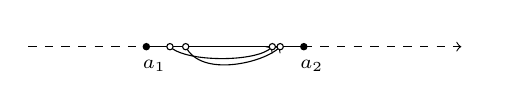
\begin{tikzpicture}
       \path (-1.5,2) coordinate (P);
       \path (4,2) coordinate (Q);
       \path (0,2) coordinate (A);
       \path (2,2) coordinate (B);
       \path (0.3,2) coordinate (M1);
       \path (1.6,2) coordinate (N1);
       \path (0.5,2) coordinate (M2);
       \path (1.7,2) coordinate (N2);
       % real line -------
       \draw [style=dashed] (P) -- (A);
       \draw (A) -- (B);
       % real line -------
       \draw [->][style=dashed](B) -- (Q) node[above right] {\scriptsize{$\R$}}; 
       % boundaries -----
       \draw (A) ++(0.1,-0.05) node[below] {\scriptsize{$a_1$}};
       \draw (B) ++(0.1,-0.05) node[below] {\scriptsize{$a_2$}};
       % circles in A and B -----
       \draw (A) [fill=black] circle (0.04);
       \draw (B) [fill=black] circle (0.04);
       % flow of the middle points ----
       \draw [->](M1)..controls (0.5,1.8) and (1.4,1.8)..(N1);
       \draw [->](M2)..controls (0.7,1.6) and (1.5,1.8)..(N2);
       % middle points -------
       \draw (M1) [fill=white] circle (0.04);
       \draw (M2) [fill=white] circle (0.04);
       \draw (N1) [fill=white] circle (0.04);
       \draw (N2) [fill=white] circle (0.04);
       \end{tikzpicture}
       \end{center}  
 Since the same is true
 for the Cayley transform, namely $\vac^{\R_+}=\vac^{\s_+}\circ C$,
 then the modular flow on the circle is nothing but
 \[
 \sigma_t^{\s_+}=C\circ\sigma_t^{\R_+}\circ C^{-1}.
 \]
 
 \bigskip
 This property ensures that the action of the modular group
 on Fermi fields localised in one interval is geometric. Now
 the question that naturally arises and that we want to address
 is what the modular group is whenever fields are localised
 in different intervals instead. As we shall see, the action
 can no more be geometric because of conflicts with algebraic
 properties otherwise. As first, we introduce the following 
 characterisation of von Neumann algebras due to Takesaki 
 \cite{Tak:1970}
 and we rephrase it in the language of nets with cyclic
 and separating vectors. 
 \begin{definition}[conditional expectation]
 Let $\mathcal{N}\subset\mathcal{M}$ be an inclusion of
 von Neumann algebras and let $\varphi$ be a cyclic and
 separating state on 
 $\mathcal{M}$. A linear map $\mathcal{E}\colon\mathcal{M}
 \to\mathcal{N}$ is called the ``conditional expectation''
 of $\mathcal{M}$ onto $\mathcal{N}$ with respect to
 $\varphi$~if
  \begin{enumerate}
   \item $\varphi\circ\mathcal{E}=\varphi|_{\mathcal{N}}$
   \item $\mathcal{E}(x)=x,\quad x\in\mathcal{N}$
   \item $\mathcal{E}(x) \Omega=P_{\I}\,x\,\Omega
          \quad x\in\mathcal{M}$
  \end{enumerate}
 where $\Omega$ emerges out of the \ac{GNS} representation
 of $\varphi$ and $P_{\I}$ projects onto
 $\hil_{\I}=\set{x\,\Omega\mid x\in\alg{\I}}$.
 \end{definition}
 \begin{theorem}[Takesaki, \cite{Tak:1970}]
 Let $\mathcal{N}\subset\mathcal{M}$ and $\varphi$ as above. 
 The existence of a conditional expectation 
 $\mathcal{E}\colon\mathcal{M} \to\mathcal{N}$ is equivalent
 to the global invariance $\sigma_t^{\varphi}(\mathcal{N})=
 \mathcal{N}$ under the modular automorphism group. 
 \end{theorem}
 Let us now assume we take two (for the sake of simplicity)
 any disjoint intervals $\I_1,\I_2\mid \I_1\cup\I_2\eqqcolon \textrm{E}_2$
 and consider the action of the modular group of the algebra
 $\alg{\textrm{E}_2}$ with respect
 to the vacuum state. The action being still 
 geometric within each of the disjoint intervals
 would imply that $\sigma_t(\alg{\I_k})\subset\alg{\I_k}$ and
 as a consequence conditions for the Takesaki's theorem would
 apply. The Reeh-Schlieder property ensures that the vacuum
 is cyclic and separating for each of the two subalgebras, hence
 the subset $\hil_{\I}$ is dense in $\hil$. Therefore $P_{\I}=
 \bm{1}$ and $\mathcal{E}\Omega=x\Omega,\,x\in\alg{\textrm{E}_2}$.
 Since $\Omega$ is also separating then $\mathcal{E}x=x$ however
 you choose $x\in\alg{\textrm{E}_2}$ and thus $\alg{\textrm{E}_2}$
 must coincide with $\alg{\I_k}$, which is not the case at hand.
 From this we realise that the action of the modular automorphism
 group (with respect to the vacuum state)
 on Fermi fields localised in disjoint intervals cannot be
 \emph{purely} geometric in order to avoid conflicts with
 Takesaki's theorem. We shall see that 
 a mixing with pointwise coefficients is 
 realised with free Fermi fields.
 
 
 
 \subsection{Geometric flow for product states}
 \label{product states}
 Of course, the situation is quite different if we choose
 states that decompose as the product of many vacuum states.
 This choice would destroy all the correlations among different
 intervals and no restrictions given by the Takesaki theorem
 would therefore apply. This issue has been investigated by 
 the authors of \cite{LMR:2009} and we shall summarise 
 here the important results. 
 
 Equipped with a net of Fermi algebras $\I\to\alg{\I}$
 the modular group with respect to the vacuum state
 acts geometrically within each interval on localised fields 
 (Bisognano-Wichmann property), the geometric flow being
 given by the subgroup $\delta_t$ of the M\"obius group preserving
 the interval (dilations on $\I=\R_+$).
 
 \bigskip
 Let $\I$ be an interval on the circle and $\textrm{E}_N=
 \sqrt[N]{\I}$ the symmetric $N$-interval generated,
 i. e. the set of all points $z$ such that $z^N\in\I$. 
 The $N^{\textrm{th}}$ covering of the M\"obius group, as introduced in
 \ref{The Moebius group}, acts on the net as
 \[
 U^{(N)}\left(\Lambda_{\I}^{-2\pi t}\right)\,
 \alg{\textrm{E}_N}\,
 {U^{(N)}\left(\Lambda_{\I}^{-2\pi t}\right)}^*
 =\alg{\delta^{(N)}_t(\textrm{E}_N)}
 \]
 where the geometric flow corresponds to the
 $n$-dilations $\delta_t^{(n)}(z)=\sqrt[n]{\delta_t(z^n)}$.
 Therefore each sub-interval is separately preserved
 by this action. If we assume the net to be split, then
 on $\textrm{E}_N=\I_1\cup\ldots\cup \I_n$ the split
 isomoprhism provides a correspondence 
 $\chi_{\textrm{E}_N}\colon\vee_{k=1}^N\alg{\I_k}\to
 \otimes_{k=1}^N\alg{\I_k}$. With the help of such
 a map we can construct a product state as follows:
 let $U(g_k)$ implement a family of diffeomorphisms acting like
 $z_k\mapsto z^N$ on each of the $\I_k$ and let $\vac$ be the
 respective vacuum state. Define now (\cite{LMR:2009})
 the Kawahigashi-Longo state on the algebra of the
 multi-intervals $\alg{\textrm{E}_N}$ 
 \begin{equation}
 \label{K-L state}
 \varphi_{\textrm{E}_N}\coloneqq 
 \left(\bigotimes_{k=1}^n \vac\circ \ad (U(g_k^{-1}))\right)
 \circ\chi_{\textrm{E}_N}.
 \end{equation}
 The modular automorphisms flow for such a product 
 state is, by construction, geometric within each 
 sub-interval of $\textrm{E}_N$, the geometric flow
 being given by the $N$-dilations:
 \[
 \sigma_t^{\varphi_{\textrm{E}_N}}
 \left(\alg{\I_k}\right)=\alg{\delta_t^{(N)}(\I_k)}.
 \]
 The same construction can be generalised to 
 non-symmetric intervals accordingly. We choose a 
 general family of diffeomorphisms $g_k\colon\I\to\I_k$
 with the property that, given $z\in\I$, then $z_k=g_k(z)\in\I_k$.
 The factorisation is then
 \[
 \varphi_{\textrm{E}_N}\coloneqq 
 \left(\bigotimes_{k=1}^n \vac\circ \ad (U(g_k))\right)
 \circ\chi_{\textrm{E}_N}
 \]
 and the modular group still acts geometrically,
 the geometric flow being now given by
 $\delta_t^{\textrm{E}_N}(z)=(g_k^{-1}\circ 
 \delta_t^{(1)}\circ g_k)(z)$ instead;
 obviously, this reduces to the square root map
 once you go back to $g_k(z)=$ brances of $\sqrt[N]{z}$. 
 However, we are going to examine the issue of non-symmetric
 intervals deeper, later on.
 
 
 \section{The result of Casini and Huerta}
 \label{ResultCH}
 We shall focus henceforth on the modular theory for Fermi fields
 localised in disjoint intervals and the prototype notation
 will be $\psi(x)\in\alg{\textrm{E}_N}$, with 
 $\textrm{E}_N=\I_1\cup\ldots\cup\I_N$. We shall also switch
 very often from the real line picture to the compact picture
 on the unit circle via Cayley transform. Natural notation
 is $\psi(x_k),\,x_k\in\I_k$ (and similarly for $z_k$ on the
 circle) to refer to a field evaluated in $\I_k$.
 
 \bigskip
 As we have seen, whenever
 we consider fields localised in different intervals the action
 of the modular automorphism group with respect to the vacuum state
 cannot be geometric because of conflicts between Takesaki's
 theorem and the Reeh-Schlieder property.
 A priori, for general space-time regions and massive fields, 
 the action of the modular group may be of any fuzzy sort.
 In fact, when conformal invariance no more holds, one cannot 
 transfer the geometric result of Bisognano and Wichmann via 
 conformal mappings and thereby the modular action has to be
 non-local. In particular the authors in \cite{Saf:2006, FigGui:1989} 
 tried to describe the Tomita operators whence the modular 
 automorphisms group comes in terms of pseudo-differential 
 operators, from which the non-local action of the modular 
 group arises. As for the modular group of a multi-interval 
 algebra with respect to the Fock vacuum in free conformal 
 theories, it will still act linearly on the free fields, 
 because the modular operator $S$ preserves the $N$-particle 
 subspaces and hence so does the Tomita operator $\Delta$.
 On the other hand, as we have just seen, it cannot preserve the
 single-interval subalgebras. If we knew that the action is pointwise,
 the most general modular flow would be of the form
 \begin{equation}
 \label{CHmatrix}
  \begin{matrix}
  \sigma_t(\psi(x_1))=&c_{11}(x_1,t)\psi(\zeta_t(x_1))\,+
                     &\ldots&+\,c_{1N}(x_N,t)\psi(\zeta_t(x_N))\\
  \vdots&\vdots&\vdots\\  
  \sigma_t(\psi(x_N))=&c_{N1}(x_1,t)\psi(\zeta_t(x_1))\,+
                      &\ldots&+\,c_{NN}(x_N,t)\psi(\zeta_t(x_N))
  \end{matrix}
 \end{equation}
 or, in a more compact notation,
 \begin{equation}
 \sigma_t \begin{pmatrix}
          \psi(x_1)\\
          \vdots\\
          \psi(x_N)\\
          \end{pmatrix}
 =        \begin{pmatrix}
          c_{11}(x_1,t)&\ldots& c_{1N}(x_N,t)\\
          \vdots&\ddots&\vdots\\
          c_{N1}(x_1,t)&\ldots& c_{NN}(x_N,t)\\
          \end{pmatrix} 
          \begin{pmatrix}
          \psi(\zeta_t(x_1))\\
          \vdots\\
          \psi(\zeta_t(x_1))\\
          \end{pmatrix}.
 \end{equation}
 where $\zeta_t(x)$ is some flow to be determined.
 Of course, once one switches to the circle picture, the 
 entries of the matrix are different. Indeed, the 
 unexpected finding by Casini and Huerta states 
 that for free Fermi fields, the modular flow is of this form.
 
 \bigskip
 The investigation of the modular automorphism group is
 then related to the evaluation of the coefficient appearing
 in \eqref{CHmatrix}. The original paper by \cite{CH:2009}
 provides the calculation of such coefficients using methods
 coming from density matrix and hamiltonian flows. It is 
 known that the time evolution generated by the modular 
 Hamiltonian $K$ of a system, with $\e^{iKt}=\Delta^{it}$  
 satisfies the \ac{KMS} property with 
 respect to the vacuum state and therefore coincides with
 its modular group (for details we refer the reader again to
 \cite{CH:2009} and references therein). Thermal states are 
 characterised by density matrices of the form $\rho\sim 
 \e^{-K}$ and correlators can be expressed as 
 $\scal{\Omega,\blank\Omega}= \tr(\rho\cdot\blank)$. 
 This brings up a relation between the Hamiltonian
 and the $n$-point functions (especially the two-point
 function) that can be used to compute the modular
 dynamics $\comm{K,\psi}$. Exponentiating the commutator
 one gets the entire time evolution $\e^{itK}\psi(x)
 \e^{-itK}$ corresponding to the modular action 
 $\sigma^t_{\vac}(\psi(x))=\Delta^{it}\psi(x)\Delta^{-it}$. 
 As a consequence the argument is that knowledge 
 of the Hamiltonian evolution 
 flow and density matrix allows, at least formally, 
 the computation of the modular automorphisms group in 
 terms of kernel of distributions. 
 
 \bigskip
 Let us consider the algebra of a Fermi field localised 
 in $N$ disjoint 
 open intervals $I_1\cup\ldots\I_N\eqqcolon\textrm{E}_N$,
 with $\I_k=\mathopen{]}a_k,b_k\mathclose{[} \subset \R$;
 we call the interval ``symmetric'' if $\I_k$ are the 
 $N^{\textrm{th}}$
 roots of an interval $\I\subset\R$ (in this case we write
 $\textrm{E}_N=\sqrt[N]{\I}$). 
 Let us introduce the following Casini-Huerta
 function $X\colon\textrm{E}_N\to\R_+$ mapping each of the
 intervals monotonously onto $\R_+$ as
 \begin{equation}
 \label{CHfunction}
 X(x)=-\prod_{k=1}^N\frac{x-a_k}{x-b_k}=
 \prod_{k=1}^N\frac{1+v_k}{1+u_k}\cdot\prod_{k=1}^N
 \frac{z-u_k}{z-v_k}
 \end{equation}
 where $z,u_k,v_k$ are the Cayley images of the points
 $x,a_k,b_k$. Each $X\in\R_+$ has exactly $N$ pre-images,
 one in each interval, and we refer to them as to
 $X_1^{-1}(X),\ldots,X_N^{-1}(X),\ X_j^{-1}(X)\in I_j$. 
 Similarly, we denote by $z_k^{-1}(X)$ the $k^{\textrm{th}}$ 
 pre-image on the circle. Moreover, this function has the
 remarkable property that in case of symmetric intervals,
 namely when $z^N\in\I$ and thus $z_k=\omega_k z\in\I_k$
 with $\omega_k^N=1$, then $X(z^N)=\mu\circ C^{-1}(z^N)$, where
 $\mu$ is a suitable M\"{o}bius function.
 
 \bigskip
 The original result by Casini and Huerta (\cite{CH:2009}
 and \cite{LMR:2009}) states that the modular automorphism
 group with respect to the vacuum state acts on Fermi field as
 \begin{multline}
 \label{MGdisj}
 \sqrt{{X_k^{-1}(X)}'}\,\sigma_t\left(\psi(X_k^{-1})\right)=\\
 \sum_{j=1}^N\,O(X,t)_{kj}\sqrt{{X_k^{-1}(\delta_t(X))}'}
 \psi\left((X_j^{-1}(\delta_t X))\right)
 \end{multline}
 where the flow $\zeta_t(X_k^{-1}(X))$ corresponds
 exactly to the geometric flow appearing in the one interval
 case
 \[ 
 \zeta_t(X_k^{-1}(X))=\delta_t(X_k^{-1}(X))=
 X_k^{-1}(\delta_t(X))
 \]
 with $\delta_t$ being the
 one parameter subgroup of M\"{o}bius transformations
 preserving the interval $\R_+$. The geometric part moving
 the points happens to be the same as in the one interval
 case, plus a mixing among different intervals occurs on 
 top of it. Of course, if one reads the modular flow in 
 terms of hamiltonian evolution, it is easy to understand
 that such an evolution usually delocalises fields in the 
 pure sense of quantum mechanics, and thus we can no more
 expect a geometric action within each subinterval.

 The matrix $O(X,t)$ appearing in \eqref{MGdisj} is an 
 orthogonal cocycle $\in \textrm{SO}(N)$ given in terms of 
 a differential equation (\cite{LMR:2009}) as 
 \begin{equation}
 \label{CHcocycle}
 \partial_tO(X,t)=O(X,t) K(\delta_t X)
 \end{equation}
 where the matrix $K(X)$ on the right hand side is
 \begin{equation}
 \label{matrix_K}
  {K(X)}_{kj}=
  \begin{cases}
  2\pi\,\dfrac{\sqrt{{X_k^{-1}(X)}'\,{X_j^{-1}(X)}'}}
  {{X_k^{-1}(X)} - {X_j^{-1}(X)}}\quad\mbox{if } k\neq j\\
  0\quad\mbox{otherwise}
 \end{cases}.
 \end{equation}
 The solution is a coboundary
 \[
 O(X,t)=O(X)^T\cdot O(\delta_t X)
 \]
 where $O(X)$ is the anti-path-ordered exponential
 \begin{equation}
 \label{anti-path}
 O(X)=\overline{P}\left(\e^{\displaystyle{-\frac{1}{2\pi}
 \int_{X_0}^X\dd X'\,K(X')}}\right).
 \end{equation}
 
 \bigskip
 As a matter of example we can carry out the explicit
 form of this matrix in the case of symmetric intervals.
 In this case, as we have seen, the related points
 $z_k\in\I_k$ are obtained by taking one of the $N^{\textrm{th}}$
 roots of $z^N$, hence $z_k=\omega^k z$, where
 $\omega=\e^{\frac{2\pi i}{N}}$ 
 is the $N^{\textrm{th}}$ root of the unity, $\omega^N=1$
 and $\omega^k=\e^{\frac{2\pi i}{N}k}$. Such points can also
 be obtained out of the Casini-Huerta uniformisation function,
 calculated for symmetric interval, after a suitable
 match with a M\"obius transformation (this is necessary
 whenever the Casini-Huerta function has range $\R_+$, to
 match the M\"obius transformation taking the upper semi-circle
 to the interval $\I$).
 
 However, the symmetric form drastically simplifies 
 the entries of the matrik $K(X)$, as they become 
 \begin{equation}
  {K(z)}_{kj}= 2\pi\,\frac{\omega^{\frac{k+j}{2}}}
  {(\omega^k-\omega^j)z}=-\overline{K}_{kj}\,\frac{1}{z}
 \end{equation}
 with $\overline{K}_{kj}$ a matrix with constant entries
 \[
 \overline{K}_{kj}=-\frac{\omega^{\frac{k+j}{2}}}
  {(\omega^k-\omega^j)};
 \]
 of course ${K(z)}_{kj}$ is still zero if $k=j$.
 Since the matrix $\overline{K}$ is a constant matrix, it
 commutes with itself at different points and as a consequence
 the anti-path-ordered exponential reduces to an ordinary
 exponential
 \begin{equation}
 O(X)=\e^{\displaystyle{\,\frac{1}{2\pi}\,2\pi\,\overline{K}
 \int_1^z \dd w\,\frac{1}{w}}}
 =\e^{\displaystyle{\,\overline{K}\ln z}}=z^{\displaystyle{\overline{K}}};
 \end{equation}
 clearly enough, $z=\e^{i\varphi}$ is any point on the
 circle. The expression we have obtained is rather simple,
 in the case of symmetric intervals; later on we will
 introduce a lemma stating the particular form allowed
 for the spectrum of such a matrix, also calculating
 the particular diagonal form it acquires after an
 orthonormal transformation $K=B^{-1}\,D\,B$, with 
 a unitary matrix $B$ and a diagonal matrix $D$. 
 For the moment we can just plug this expression in the 
 above formula (no matter what these matrices actually are)
 to obtain 
 \[
 z^{\displaystyle{\overline{K}}}=
 z^{\displaystyle{B^{-1}\,D\,B}}=
 \e^{i\varphi\displaystyle{B^{-1}\,D\,B}}=
 B^{-1}\,z^{\displaystyle{D}}\,B
 \]
 and the matrix $D$ can be decomposed over its 
 eigenvalues $\lambda_k$ as $D=\sum_{k=1}^{n}
 \lambda_k\,P_k$, where $P_k\coloneqq \ket{e_k}\bra{e_k}$ 
 is the projection over the $k^{\textrm{th}}$ eigenspace.
 Running once around the circle the change in the variable 
 $z$ is $z\mapsto \e^{2\pi i}z$ and so the matrix $O(z)$
 changes consequently as
 \[
 O(\e^{2\pi i}z)=B^{-1}\,\e^{2\pi i\,
 \displaystyle{\sum_{k=1}^n\lambda_k P_k}}
 \,z^{\displaystyle{\overline{K}}}\,B.
 \]
 We shall see that the spectrum $\lambda_k$ of $D$
 is basically made of natural numbers so that eventually
 one obtains $\e^{(N+1)i\pi}$ and thus we 
 conclude that the only change in the matrix $O(z)$ 
 is up to a minus sign: $O(\e^{2\pi i}z)=(-1)^{N+1}\,O(z)$.
 
 \bigskip
 As we mentioned, the spectrum of the matrix $K(X)$ is 
 given, in the symmetric case, by the following:
 \begin{lemma}[\cite{Rehren:2012wa}]
 The matrix $K(X)$ has integer spaced spectrum 
 $\frac{1-n}{2},\ldots,\frac{n-1}{2}$ in the symmetric
 case. It is diagonalised by the unitary matrix 
 $\frac{1}{\sqrt{n}}B$ whose entries are 
 $B_{kj}=\omega^{(1/2-k)j}$, $\omega$ being given
 by the root of the unity as above. This implies 
 $B\,K=D\,B$, where $D$ is the diagonal matrix
 with entries $D_{kk}=\frac{n+1}{2}-k$.
 \end{lemma}
 \begin{proof}
 By direct computation of the left hand side 
 \begin{multline*}
 \sum_{j\neq l}^n B_{kj}K_{jl}=-
 \sum_{j=l+1}^{n+l-1}\frac{\omega^{(1/2-k)j}
 \omega^{\frac{j+l}{2}}}{\omega^j-\omega^l}\\
 =-\omega^{(1/2-k)l}\sum_{j=1}^{n-1}
 \frac{\omega^{(1/2-k)j}\omega^{\frac{j+2l}{2}}}{(\omega^j-1)\omega^l}
 \end{multline*}
 where we made use of the invariance of the sum under 
 the shift $j\to j+n$. Now we symmetrise again the 
 sum under $j\leftrightarrow n-j$ to have 
 \begin{multline*}
 \sum_{j\neq l}^n B_{kj}K_{jl}=
 -B_{kl}\sum_{j=1}^{n-1}\frac{\omega^{(1-k)j}}{\omega^j-1}\\
 =-B_{kl}\cdot \frac{1}{2}\sum_{j=1}^{n-1}
 \Big(\frac{\omega^{(1-k)j}}{\omega^j-1}+
 \frac{\omega^{(1-k)(n-j)}}{\omega^{n-j}-1}\Big)
 \end{multline*} 
 \noindent Notice now that whenever $z\in\s$ 
 is a phase, contributions of the form 
 \[
 \frac{z^m-z^{-m}}{z-z^{-1}}=z^{m-1}+\ldots 
 +z^{1-m}
 \]
 can be simplified cancelling the denominators. 
 This applies as well to $\omega$ and the 
 right hand side becomes then 
 \[
 -B_{kl}\cdot\frac{1}{2}\sum_{j=1}^{n-1}
 \frac{\omega^{(1-k)j}-\omega^{kj}}{\omega^j-1}
 =B_{kl}\cdot\frac{1}{2}\sum_{j=1}^{n-1}
 \sum_{\nu=1-k}^{k-1}\omega^{j\nu}.
 \]
 Since $\omega^n=1$ we derive that 
 $\sum_{j=0}^n\omega^{j\nu}=n\,\delta_{\nu,0}$
 and thus 
 \[
 \sum_{j\neq l}^n B_{kj}K_{jl}=
 B_{kl}\sum_{\nu=1-k}^{k-1}(n\,\delta_{\nu,0}-1)
 =B_{kl}\cdot\frac{1}{2}(n-2k+1)=D_{kk}\cdot B_{kl}
 \]
 completing the proof.
 \end{proof}


 
 \section{Diffeomorphisms covariance}
 \label{Longo-Xu}
 We shall now turn to a very important feature 
 of conformal nets on the circle which follows 
 from the way fields are assumed to transform 
 under diffeomorphisms. We shall follow the guide 
 lines provided by \cite{LX:2004}: we assume the net
 to be diffeomorphisms covariant and split, i. e.
 for each couple of intervals $\I_1,\I_2$ with 
 disjoint closure, there exist an isomoprhism 
 (the ``split map'') $\chi\colon\alg{I_1}\vee
 \alg{I_2}\to\alg{I_1}\otimes\alg{I_2}$ such that
 $\chi(a_1 a_2)=a_1\otimes a_2$, however you choose
 $a_1\in \alg{\I_1},a_2\in\alg{\I_2}$.
 
 \bigskip 
 Let now $\I$ be an interval on the circle and
 denote as $\mathcal{A}^N(\I)=\alg{\I}\otimes\ldots 
 \otimes\alg{\I}$ many copies of the related algebra.
 We introduce a family of diffeomorphisms 
 $\gamma_j\colon\I\to\I_j$ such that, with natural 
 understanding of notations, given $z\in\I$ then 
 $\gamma_j(z)=z_j\in \I_j$. Diffeomorphisms covariance
 implies the existence of a continuous 
 projective unitary representation of $\Diff(\s)$.
 Once we choose the $\gamma_j$ their action 
 is implemented on the net by means of unitaries 
 $U(\gamma_j)$:
 \[
 \phi^j_I\coloneqq\left.\ad U(\gamma)\right|\alg{\I}=
 \alg{\gamma_j(\I)}=\alg{\I_j}
 \]
 in this respect $\phi^j_I$ is an isomoprhism 
 $\phi^j_I\colon\alg{\I}\to\alg{\I_j}$. Therefore 
 taking the tensor product $N$ times we obtain a map
 \[
 \bigotimes_{k=1}^N \phi_I^k=\phi_I^1\otimes\ldots\otimes
 \phi_I^n\colon\mathcal{A}^N(\I)\to\alg{\I_1}\otimes
 \ldots\otimes\alg{\I_N}
 \]
 acting on the elements as $\phi_I^1(a_1)\otimes\ldots\otimes 
 \phi_I^N(a_N)$. We can now compose everything with 
 the inverse split map $\chi^{-1}$ at our disposal 
 in order to bring $\alg{\I_1}\otimes\ldots\otimes\alg{\I_N}$ 
 into $\alg{\I_1\cup\ldots\cup\I_N}$. The assignment we 
 eventually obtain is called the Longo-Xu map 
 \begin{equation}
 \label{L-X}
 \LX\colon\mathcal{A}^N(\I)\to\mathcal{A}
 (\I_1\cup\ldots \cup\I_N)
 \end{equation}
 and it is explicitly realised on the elements as
 \begin{align*}
 \LX(a_1\otimes\ldots\otimes a_N)&\coloneqq
 \left(\chi^{-1}\circ\bigotimes_{k=1}^N \phi_I^k\right)
 (a_1\otimes\ldots\otimes a_N)\\[1.5ex]
 &=\phi_I^1(a_1)\cdot\ldots\cdot\phi_I^N(a_N) 
 \end{align*}
 for each $a_1,\ldots,a_N\in\alg{\I}$. As a matter
 of example, and very useful for the forthcoming
 purposes, we shall give the explicit formulae
 for the Longo-Xu map in case the diffeomorphisms
 $\gamma_j(z)$ coincide with the inverse root map.
 \begin{example}[Square root map]
 For the sake of simplicity let us restrict to a 
 symmetric two-interval $\sqrt{\I}=\I_1\cup\I_2$, 
 that is the
 set of points $z\in\s$ such that $z^2\in\I$. 
 The diffeomorphism at hand is the square root 
 map $z^2\mapsto \sqrt{z^2}=\pm z$ and we identify
 the two solutions as the two branches $\mu_1(z^2)=
 z$, $\mu_2(z^2)=-z$ and thus the two intervals are
 related to each other as $\I_2=\rot(\pi)(\I_1)$. Also,
 in order to avoid troubles with the discontinuities,
 we require such interval not to contain the point 
 where the cut in the square root is chosen. \\
 
 In particular, if we take two copies $\psi^{(1)},
 \psi^{(2)}$ of a Fermi field localised in $\I$ we have,
 applying \eqref{L-X}
 \begin{align*}
 \LX\left(\psi^{(1)}(z^2)\otimes\bm{1}\right)&=
 \ad U\left(\sqrt{\blank}\right)(\psi^{(1)}(z^2))\cdot\bm{1}\\
 \LX\left(\bm{1}\otimes\psi^{(2)}(z^2)\right)&=
 \bm{1}\cdot\ad U\left(-\sqrt{\blank}\right)(\psi^{(2)}(z^2)).\\ 
 \end{align*}
 By using the conformal transformation law of the 
 Fermi fields, the adjoint action reduces to 
 \[
 \ad U(\gamma)\psi(z)=\sqrt{\frac{\partial\gamma}{\partial z}}
 \,\psi(\gamma(z))
 \] 
 and thus
 \begin{align*}
 \LX\left(\psi^{(1)}(z^2)\otimes\bm{1}\right)&=
 \frac{1}{\sqrt{2z}}\,\psi(z)\\[1.5ex]
 \LX\left(\bm{1}\otimes\psi^{(2)}(z^2)\right)&=
 \frac{i}{\sqrt{2z}}\,\psi(-z).
 \end{align*}
 Even more useful for the next issues is the form this
 map acquires on the complex fermion 
 \begin{align}
 \LX(\phi(z^2))&=\LX\left(\psi^{(1)}(z^2)+i\psi^{(2)}(z^2)\right)
 =\frac{1}{2\sqrt{z}}\left(\psi(z)+\psi(-z)\right)
 \label{LX_complex}\\ 
 \LX(\phi(z^2)^*)&=\LX\left(\psi^{(1)}(z^2)-i\psi^{(2)}(z^2)\right)
 =\frac{1}{2\sqrt{z}}\left(\psi(z)-\psi(-z)\right).
 \end{align}
 \end{example}
 
 \bigskip
 The Longo-Xu map allows us to
 simplify the expression of the Kawahigashi-Longo
 state that we have introduced before, \eqref{K-L state}. 
 In fact, again 
 in case of a symmetric two-interval $\sqrt{I}$, 
 the state \eqref{K-L state} appears to be exactly
 \begin{align*}
 \varphi_{\sqrt{\I}}&=\left(\vac\otimes\vac\right)
 \circ\left(\ad U(z\mapsto z^2)\otimes\ad U(-z\mapsto z^2)\right)
 \circ\chi^{-1}_{\sqrt{\I}}\\ 
 \varphi_{\sqrt{\I}}&=\left(\vac\otimes\vac\right)\circ
 \LX^{-1}
 \end{align*}
 This relation is going to be very useful to compare
 such product state with the vacuum state defined 
 on the algebra of the multi-interval.
 
 \section{A multi-local isomorphism}
 \label{A multi-local isomorphism}
 In this section we present a simple isomorphism between 
 the algebra of one real chiral Fermi field and the algebras 
 of $n$ real chiral Fermi fields in the context of 
 nets of von Neumann algebras. Unlike the Longo-Xu map, 
 this isomorphism preservers
 the vacuum state due to a suitable change of localisation;
 we first prove the result for symmetric intervals and 
 then extend it to the general case of non-symmetric intervals,
 using insights and results from \cite{CH:2009}.
 
 \bigskip
 As a start-up we recall that in general, due to the
 split property, we can make use of the 
 split map between any two algebras $\chi\colon\alg{\I}\vee
 \alg{\textrm{J}}\to\alg{\I}\otimes\alg{\textrm{J}}$
 taking $ab\to a\otimes b$. To be more precise, since we
 shall be dealing with Fermi fields, the tensor product
 $\otimes^t$ is understood to be ``graded'', namely 
 for any two operators $A\otimes^t B$ is the true tensor
 product $A\otimes B$ if either of them is a Bose field, and a 
 twisted tensor product $A\otimes (-1)B$ if both of them 
 are Fermi fields. This is to ensure the correct commutation 
 or anti-commutation relations, respectively. Of course,
 whenever we are dealing with sums of 
 Bose and Fermi fields, the correct formulae for the tensor 
 product follow by linearity.
 
 However, as shown in the previous paraghraph, this is 
 implemented on the algebras as the Longo-Xu map, especially 
 when the fields at hand satisfy diffeomorphisms covariance. 
 Roughly speaking, this allows us to move the fields around the 
 circle and in particular we can bring any number $N$ of 
 ``copies'' of one algebra $\mathcal{A}^N(\I)$ onto 
 one ``delocalised'' copy of the same algebra 
 $\alg{\I_1\cup\ldots\cup\I_N}$ via 
 $\LX(a_1\otimes\ldots\otimes a_N)=
 \phi_I^1(a_1)\cdot\ldots\cdot\phi_I^N(a_N)$.
 It is nevertheless clear though, that such a map does not
 preserve the vacuum state, because product states do
 destroy correlations between fields at different points,
 $\vac(a(x)b(y))\neq \vac(a(x))\cdot\vac(b(y))$. 
 
 The new idea is that, nonetheless, a vacuum preserving 
 isomorphism does exist, it just has to be prepared ad hoc,
 and, interestingly enough, we shall see eventually that it 
 is strongly connected to the Longo-Xu isomorphism 
 through a general gauge transformation. Also, this new 
 isomorphism will be globally defined thanks to its 
 extension to the entire circle. Anyway, before we start we 
 recall once more the standard notations to be used.
 
 \bigskip 
 Let $\mathcal{A}^N(\I)$ denote $N$ copies of an algebra 
 of fields localised in the interval $\I$ on the circle 
 (likewise on the real line, we shall switch the two pictures 
 very often), i. e. $\alg{\I}\otimes\ldots\otimes\alg{\I}$.
 Whenever no representation is explicitly stated we assume 
 the fields to be in their defining vacuum representation, namely 
 $\pi_0(\alg{\I})$. However, we will try to be clear enough 
 throughout. A symmetric interval is essentially an 
 $N^{\textrm{th}}$ root $\sqrt[N]{\I}=\I_1\cup\ldots\cup
 \I_N$ and, with clear understanding of symbols, we 
 refer to $z^N\in\I$ and $z_1,\ldots,z_N$ as the roots 
 in each sub-interval $\I_k$, each of them satisfying 
 $z_k^N=z^N\in\I$. Even clearer is the following 
 notation: the related points $z_k$ can be written 
 as $z_k=\omega^k z$ if $\omega=\e^{\frac{2\pi i}{N}}$
 and $z=\e^{i\varphi}$ is any fixed point $\in \textrm{E}_N$.
 This will ensure that each of those roots 
 ``squares'' to $z^N\in\I$. In the special case of $N=2$
 this reduces to $z^2\in\I$ and $\I_1\cup\I_2$ is the 
 set of points of the form $z,-z$ as the two solutions 
 to $\sqrt{z^2}$.
 
 A non-symmetric interval $\textrm{E}_N$, instead, 
 is simply the union of any $N$ intervals with disjoint closure, 
 wherein the related points $z_k\in\I_k$ need not be 
 roots of $z^N$, rather they are defined as roots 
 of a particular $N$-folded map taking the interval 
 $\I$ onto $\I_1\cup\ldots\cup\I_N$, where each of the 
 $z_k$ appears as one of the solutions of this equation.
 In particular, this assignment will be achieved by means 
 of the Casini-Huerta function \eqref{CHfunction} whose 
 properties have already been stated.  
 
 \bigskip 
 Fields will be considered both on the real line $\R$ and
 on the circle $\s$, the passage from either picture to
 the other being achieved by means of the Cayley
 transform. Conformal fields will consequently change 
 as (the extra factor $i$ is conventional)
 \[
 \phi(z)=\sqrt{-i\frac{dz}{dx}}\,\phi(x)=
 \frac{1-ix}{\sqrt{2}}\,\phi(x).
 \]
 Fields in the compact picture are just a reparametrisation
 of fields on the real line, and the extension to the 
 entire circle depends on the representation. As already 
 introduced in the previous paraghraph 
 \ref{repn of Fermi on the circle}, Fermi fields on the real 
 line posses two faithful representations: the vacuum (Neveu-
 Schwarz) and the Ramond representation, the former extending 
 periodically on the circle, the latter anti-periodically.
 The starting point will be a real chiral Fermi field versus 
 two copies thereof, also seen as a complex fermion again in the 
 sense of \ref{repn of Fermi on the circle}, where all the notations,
 two-point functions and commutation rules have already been 
 stated. Obviously fields must be smeared with suitable 
 functions in order to obtain operators on a Hilbert space;
 nevertheless most of the computations will be clear in the 
 sense of distribution, if not stated otherwise.
 
 Moreover, due to the fact that the fields are assumed to be 
 free (and hence their anti-commutators are multiples of the 
 identity operator) the standard anti-commutation relations 
 can be recovered out of the two-point function as 
 \begin{multline*}
 \omega(\psi(z)\psi(w))+\omega(\psi(w)\psi(z))=
 \omega(\omega(\psi(z)\psi(w))+\\ 
 \omega(\psi(w)\psi(z)))=
 \omega(\ant{\psi(z),\psi(w)})=\ant{\psi(z),\psi(w)}.
 \end{multline*}
 In the case at hand we recover
 \[
 \ant{\psi(z),\psi(w)}=\lim_{\lambda\to 1}
 \left(\frac{1}{z-\lambda w} +\frac{1}{w-\lambda z} \right)=
 \frac{2\pi}{z}\,\delta(\varphi-\theta)
 \]
 if $z=\e^{i\varphi}$ and $w=\e^{i\theta}$, for
 $\varphi,\theta\in\open{-\pi}{\pi}$.
 
%*****************************************
\subsection{The symmetric case}
\label{beta symmetric}
%*****************************************
We start with the symmetric case for $N=2$,
namely $z^2\in\I$ and $z,-z\in\I_1,\I_2$ 
respectively. A complex Fermi field $\phi(z^2),
\phi^*(z^2)$ is localised in $\I$ and a real 
Fermi field $\psi(z)$ in $\sqrt{\I}=\I_1\cup 
\I_2$.
\begin{proposition}[\cite{Rehren:2012wa}]
Let $\phi$ and $\psi$ stand for the complex and real 
fermion in their vacuum representation, as stated 
above. The linear map 
\begin{equation}
\label{beta}
\beta\colon\mathcal{A}^2(\I)
\to\alg{\sqrt{I}}
\end{equation}
given by 
\begin{align}
\phi(z^2)&\mapsto\frac{1}{2}
\left(\psi(z)+\psi(-z)\right)
\label{beta_complex}\\[1ex]
\phi^*(z^2)&\mapsto\frac{1}{2z}
\left(\psi(z)-\psi(-z)\right)
\end{align}
for $z\in\s$, induces an isomorphism of $\textrm{CAR}$
algebras preserving the vacuum state on the different 
algebras: $\vac^{(1)}\circ\beta=\vac^{(2)}$. Note that 
the map is well defined because the right hand sides
are invariant under $z\mapsto -z$.
\end{proposition}
\begin{proof}
We start showing the inverse of such a map: clearly, 
summing up the two sides of the equations we obtain
\begin{align*}
2\,\psi(z)&=2\,\beta(\phi(z^2)) + 2z\,\beta(\phi^*(z^2))\\
2\,\psi(-z)&=2\,\beta(\phi(z^2)) - 2z\,\beta(\phi^*(z^2))\\
\end{align*}
therefore the inverse relation reads
\[
\beta^{-1}\left(\psi(\pm z)\right)=\phi(z^2)\pm z\phi^*(z^2).
\]
The adjoint relation is immediate:
\[
\beta(\phi(z^2))^*=z^2\,\beta(\phi^*(z^2)),
\]
hence $\beta$ preserves the adjoints too.
In terms of the two copies 
$\phi(x)=\left(\psi_1(x)+i\psi_2(x)\right)/\sqrt{2}$
the map $\beta$ can be written as
\begin{align*}
\psi_1(z^2)&\mapsto\frac{1}{2\sqrt{2}}\,\psi(z)
\left(1+\frac{1}{z}\right)+\frac{1}{2\sqrt{2}}\,\psi(-z)
\left(1-\frac{1}{z}\right)\\[1ex]
\psi_2(z^2)&\mapsto\frac{1}{2\sqrt{2}}\,\psi(z)
\left(1-\frac{1}{z}\right)+\frac{1}{2\sqrt{2}}\,\psi(-z)
\left(1+\frac{1}{z}\right)\\
\end{align*}
with inverse given by
\[
\beta^{-1}\left(\psi(\pm z)\right)=\
\psi_1(z^2)(1\pm z) +i\psi_2(z^2)(1\mp z).
\]
Now we turn to the vacuum preserving features. The 
simplest proof proceeds by brute force plugging the 
right hand side of \eqref{beta} into the two-point 
function and evaluating the result:
\begin{align*}
\vac\circ\beta\left(\phi^*(z^2)\phi(w^2)\right)&=
\vac\left(\beta(\phi^*(z^2))\beta(\phi(w^2))\right)\\
&=\vac\left(\frac{1}{2z}(\psi(z)-\psi(-z))\right. \cdot
\left.\frac{1}{2}(\psi(w)+\psi(-w))\right)
\end{align*}
this brings four contributions:
\begin{multline*}
\frac{1}{4z}\left(\vac(\psi(z)\psi(w))-\vac(\psi(-z)\psi(w))\right. \\
+\left. \vac(\psi(z)\psi(-w))-\vac(\psi(-z)\psi(-w))\right)
\end{multline*}
which can be summed up using the formula for the vacuum 
two-point function for the real chiral Fermi field 
\begin{align*}
\vac\circ\beta\left(\phi^*(z^2)\phi(w^2)\right)&=
\frac{1}{4z}\left( \frac{1}{z-w}-\frac{1}{-z-w}\right. 
+\left. \frac{1}{z+w}-\frac{1}{-z+w}\right)\\
&=\frac{1}{4z}\,2\,\left(\frac{1}{z-w}+\frac{1}{z+w}\right)\\
&=\frac{1}{2z}\cdot\frac{2z}{z^2-w^2}=\frac{1}{z^2-w^2}\\
&=\vac\left(\phi^*(z^2)\phi(w^2)\right)
\end{align*}
as to be proven. By exploiting Wick theorem, this 
equality extends to all $n$-points functions, since 
these are just sums of products of two-point functions,
see equation \eqref{wick}. As already pointed out, the 
standard anti-commutation relations follow from this
correlation function, therefore they remain preserved as
well.

\bigskip 
Another proof proceeds by simply looking at Fourier modes. 
In the vacuum representation, where we assume the fields are 
evaluated, we have 
\[
 \phi(z^2)=\sum_{r\in\Z+1/2}\phi_r\,
 {(z^2)}^{-r-1/2},\quad
 \psi(z)=\sum_{r\in\Z+1/2}\psi_r\,
 z^{-r-1/2}.
\]
A simple look at the right hand sides of \eqref{beta} 
displays that, for example,
\begin{align*}
\beta\left(\phi(z^2)\right)&=\sum_{r\in\Z+1/2}\beta(\phi_r)\,
 {(z^2)}^{-r-1/2}=
\frac{1}{2}\left(\psi(z)+\psi(-z)\right)\\[1ex]
&=\frac{1}{2}\sum_{r\in\Z+1/2}\phi_r\,z^{-r-1/2}
\left(1+(-1)^{-r-1/2}\right) \\[1ex]
&=\sum_{p\in\Z}\psi_{2p-1/2}{(z^2)}^{-p}=
\sum_{r\in\Z+1/2}\psi_{2r+1/2}{(z^2)}^{-r-1/2}
\end{align*}
therefore the isomorphism appears as a relabelling 
of the Fourier modes $\phi_r\mapsto\psi_{2r+1/2}$.
Similarly for the adjoint field we have 
$\phi^*_r\mapsto\psi_{2r-1/2}$; the variable $r$
runs into $\Z+1/2$ for the vacuum representation.
In terms of these Fourier modes the anti-commutation
relations read
\[
\ant{\phi_r,\phi^*_s}=\ant{\psi_r,\psi_s}=\delta_{r+s,0}
\]
and a simple look shows that
\[
\ant*{\beta(\phi_r),\beta(\phi^*_s)}=
\ant{\psi_{2r+1/2},\psi_{2s-1/2}}=\delta_{2r+1/2+2s-1/2,0}
=\delta_{r+s,0};
\]
the vacuum state is the only state which is annihilated 
by all $\psi_r, r>0$ and by all $\phi_r,\phi_r^*, r>0$,
respectively. Of course the relabelling does not 
change these conditions and ergo the vacuum is still sent 
into itself. The adjoint relations in terms of modes are
$\phi_r^*=(\phi_{-r})^*$ and we can easily see that, by 
making use of $\beta(\phi(z^2))^*=z^2\,\beta(\phi^*(z^2))$
multiplication by $z^2$ becomes a shift by $-1$ in terms 
of modes, and this is exactly $2r+1/2-1=2r-1/2$, indeed 
what happens to $\phi^*_r$ under the action of $\beta$.

\bigskip 
We have thus shown that $\beta$ is an isomorphism that 
preserves the vacuum state, both in the ``local'' setting
(by looking at the two-point function) and from the 
algebraic perspective of anti-commutators.
This is due to change of localisation from the point 
$z^2$ to the points $z,-z$ with suitable coefficients that
must adjust the form of two-point function eventually. We shall 
see later on that such coefficients will acquire a more
general form described by the Casini-Huerta function 
\eqref{CHfunction} in the context of modular theory and this 
will come as a very special feature; with any other function 
$\I_k\to \I$ the statement is no more true. The 
reduction to special symmetric case brings back the form 
we have just analysed. However, it is 
interesting to show what the map $\beta$ becomes on the 
real line, instead. Since $\R=C^{-1}(\s\setminus\set{-1})$ 
then 
\[
\beta^{\R}=C^{-1}\circ\beta^{\s}\circ C.
\]
The square root assignment $z^2\mapsto\sqrt{z^2}=\pm z$
becomes, after Cayley transform, 
$C^{-1}(z^2)=q(x)=2x/(1-x^2)$, whose two 
``square roots'' are the points $x=C^{-1}(z)$ and
$-1/x=C^{-1}(-z)$.
We have that, on the real line, $\beta^{\R}$ is
\begin{align*}
\phi(q(x))&\mapsto\frac{1}{q(x)}\cdot\frac{1}{1-ix}
\Big(x\psi(x)+i\psi(-1/x)\Big)\\
\phi^*(q(x))&\mapsto\frac{1}{q(x)}\cdot\frac{1}{1+ix}
\Big(x\psi(x)-i\psi(-1/x)\Big)
\end{align*}
and the inverse relation is simply
\[
\beta^{-1}(\psi(x))=\frac{1-ix}{1-x^2}\,\phi(q(x)) +
\frac{1+ix}{1-x^2}\,\phi^*(q(x)).
\]
One might still ask to show why the vacuum correlation 
function is preserved on the real line too; this can be
easily proven by brute force, though we prefer to show a
more elegant solution as follows: the vacuum states on the 
real line and on the circle are related via $\vac^{\R}=
\vac^{\s}\circ C$:
\begin{align*}
\vac^{\R}\circ\beta^{\R}&=\vac^{\s}\circ C\circ\beta^{\R}\\
&=\vac^{\s}\circ C\circ C^{-1}\circ\beta^{\s}\circ C\\
&=\vac^{\s}\circ\beta^{\s}\circ C\\
&=\vac^{\s}\circ C=\vac^{\R}
\end{align*}
as to be proven. \qedhere
\end{proof}
With a little care the result we have just presented can be 
straightforwardly generalised to the case of symmetric $N$-intervals. 
Before we do so, we notice that
a closer look to $\beta$ brings the following inspection to 
the coefficients appearing on the right hand sides:
\begin{align*}
\phi(z^2)&\mapsto \frac{z^0}{2}
\left(\psi(\omega^0 z)+\psi(\omega^1 z)\right)\\
\phi^*(z^2)&\mapsto \frac{z^{-1}}{2}
\left(\psi(\omega^0 z)-\psi(\omega^1 z)\right)
\end{align*}
where we have introduced the roots of the unity $\omega^{0,1}=\pm 1$
as in the fashion previously described. Even more compact
is the form:
\begin{equation*}
\phi^{(k)}(z^2)\mapsto\frac{z^{1-k}}{N}\,\sum_{j=0}^{N-1}
\omega^{(1-k)j}\,\psi(\omega^j z)\qquad k=1,2.
\end{equation*}
Let us now take any symmetric $N$-interval with arbitrary $N$, 
exploiting the form of $\sqrt[N]{z^N}$ with $N$
solutions $z_1,\ldots,z_N$ such that $z_k=\omega^k z\in\I_k$.
Similarly we choose $N$ real Fermi fields lying in $\alg{\I}$ 
which we can pairwise combine into $N/2$ complex Fermi fields:
in formulae we assign $\psi^{(1)}(z^N),\ldots,\psi^{(N)}(z^N)$
such that ${{\phi^{(k)}}^*(z^N)}=\phi^{(N+1-k)}(z^N)$.
Then we just have to propose the same ansatz 
for a symmetric $N$-interval $\beta\colon
\mathcal{A}^N(\I)\to\alg{\sqrt[N]{\I}}$
\begin{equation}
\label{beta_any}
\phi^{(k)}(z^2)\mapsto\frac{z^{1-k}}{N}\,\sum_{j=0}^{N-1}
\omega^{(1-k)j}\,\psi(\omega^j z)\qquad k=1,\ldots,N.
\end{equation}
In terms of the initial fields and in terms of Fourier 
modes this becomes 
\[
\psi^{(k)}(z^N)\mapsto\sum_{r\in\Z+1/2}\psi_{1/2-k + (r+1/2)N}\,
{(z^N)}^{-r-1/2}
\]
which corresponds in turn to a relabelling 
of generators $\psi^{(k)}_r\mapsto\psi_{1/2-k + (r+1/2)N}$.
That this is still a vacuum preserving isomorphism can be
again verified by noting that the renumbering of generators 
does not affect the vacuum, or by direct computation of the 
two-point functions, along the same lines as before.







%*****************************************
%*****************************************
%*****************************************
%*****************************************
%*****************************************

%*****************************************
\subsection{The Ramond sector}
\label{The Ramond sector}
%*****************************************
The real free Fermi field possesses another faithful 
representation of positive energy, the Ramond 
sector, as we have seen in \ref{repn of Fermi on the circle}, 
induced by the \ac{GNS} construction from the 
two-point function \eqref{Ramond}. Fields evaluated
in the Ramond sector will be expressed as 
$\ram{z}$. Obviously, as previously stated, their 
representation on the circle in terms of Fourier modes
has a cut at $z=-1$ and extends anti-periodically on the 
whole $\s$:
\[
\ram{z}=\sum_{n\in\Z}{\psi_{\textrm{R},}}_n \,z^{-n-1/2}.
\]
In principle one could just introduce a new field obtained 
by multiplying the actual Ramond field by $\sqrt{z}$, 
in order to ``cancel'' the cut: $\ram{z}\mapsto 
\sqrt{z}\cdot\ram{z}$ and so 
\[
\ram{z}=\sum_{n\in\Z}{\psi_{\textrm{R},}}_n \,z^{-n}
\]
with two-point function
\[
\omega_{\textrm{R}}(\ram{z}\ram{w})=
\frac{1}{2}\cdot\frac{z+w}{z-w}.
\]
Indeed, if we do so, the transformation law for the new 
defined conformal field under diffeomorphisms 
$z\mapsto \gamma(z)$ changes by an extra factor of $\sqrt{z/\gamma(z)}$.
Commutation relations between modes have the form 
$\ant{{\psi_{\textrm{R},}}_n,{\psi_{\textrm{R},}}_m}
=\delta_{n+m,0}$. In particular, the zero mode squares
to one: $2{\psi^2_{\textrm{R},}}_0=\bm{1}$.

\bigskip 
\begin{proposition}
A similar isomorphism like in \eqref{beta} can be 
introduced as 
\begin{equation}
\label{beta_ramond}
\beta_{\textrm{R}}\colon\pi_0(\alg{\I})\otimes^t 
\pi_{\textrm{R}}(\alg{\I})\to
\pi_{\textrm{R}}\left(\alg{\sqrt{I}}\right)
\end{equation}
taking the tensor product of fields in the vacuum and in 
the Ramond sector and defining
\begin{align}
\ram{z^2}\otimes^t\bm{1}_0&\mapsto\frac{1}{2}
\Big(\ram{z}+\ram{-z}\Big)\\[1ex]
\bm{1}_{\textrm{R}}\otimes^t\pi_0(\psi(z^2))&\mapsto\frac{1}{2z}
\Big(\ram{z}-\ram{-z}\Big).
\end{align}
This isomorphism still preserves the vacuum state in the 
form $\omega_{\textrm{R}}\circ\beta_{\textrm{R}}=
\omega_{\textrm{R}}\otimes\vac$.
\end{proposition}
\begin{proof}
We look again at the Fourier modes and the right hand 
sides present a relabelling ${\psi_{\textrm{R},}}_n\mapsto 
{\psi_{\textrm{R},}}_{2n}$ and ${\psi_{\textrm{R},}}_n\mapsto 
{\psi_{\textrm{R},}}_{2n+1}$, respectively;
this ensures that the correct commutation relations 
and two-point function directly follow.\qedhere
\end{proof}











%*****************************************
%*****************************************
%*****************************************
%*****************************************
%*****************************************
%*****************************************
\subsection{The non-symmetric case}
\label{beta non-symmetric}
%*****************************************
We turn now the attention to the vacuum representation in 
the non-symmetric case 
and try to follow the same arguments as before, in 
order to figure out whether an analogous map, 
playing the role of $\beta$, can be derived for 
non-symmetric intervals.
As we said, we take $\textrm{E}_N$ to be any union
of $N$ disjoint intervals on the real line (likewise
on the circle via Cayley map); thus we are looking for 
\begin{equation}
\label{beta_non-sym}
{\beta}'\colon\mathcal{A}^N(\I)\to\alg{\textrm{E}_N}
\end{equation}
that still preserves the vacuum state
$\vac^{(N)}\circ\beta=\vac\otimes\cdots\otimes\vac$. 

For $N=2$ every non-symmetric two-interval can be 
obtained by applying a M\"obius transformation $\mu$ on a 
symmetric one. Therefore the generic 
$\beta'_2$ is nothing but $\mu\circ\beta_2$ and the vacuum 
preservation is ensured by the fact that any M\"obius 
transformation preserves itself the vacuum state. This 
result in no more true for $N\neq 2$ and in the general 
case we need arguments coming from modular theory to
help our constructions.

\bigskip 
In order to introduce such a map we briefly recall a 
general result: let the intervals be given by 
$\I_k=\mathopen{]}a_k,b_k\mathclose{[} \subset \R$ and define 
the function $X(x),\,x\in \R$ by
\begin{equation}
\label{CHfunction}
X(x) = - \prod_{k=1}^N \frac{x-a_k}{x-b_k}\,.
\end{equation}
This function maps each interval monotonously onto $\R_+$, 
so that every $X\in \R_+$ happens to have exactly $n$ 
pre-images (which we refer to as $X_1^{-1}(X),\ldots,X_n^{-1}(X)$), 
one in each interval, $X_j^{-1}(X) \in I_j$.
We borrow the formulae appearing in \cite{CH:2009} 
for reasons that will become clear later. 
In particular, we look at the 
form of the modular automorphisms group for Fermi fields
localised in disjoint intervals, equation \eqref{MGdisj}
 \begin{multline*}
 \sqrt{{X_k^{-1}(X)}'}\,\sigma_t\left(\psi(X_k^{-1})\right)=\\
 \sum_{j=1}^N\,O(X,t)_{kj}\sqrt{{X_k^{-1}(\delta_t(X))}'}
 \psi\left((X_j^{-1}(\delta_t X))\right).
 \end{multline*}
Here fields are evaluated on the real line as functions 
of the variable $X\in\R_+$. We thus have a collection 
of $N$ fields: $\psi_1(X),\ldots,\psi_N(X)$. The 
map $\beta'$ is explicitly given by
\begin{equation}
\label{map_beta_general}
\beta'(\psi_i(X))= \sum_{r=1}^N {O(X)}_{ir}\,\sqrt{{X_r^{-1}(X)}'}\ 
\psi(X_r^{-1}(X))
\end{equation}
where the mixing matrix $O(X)$ is the solution of 
\eqref{CHcocycle} given in terms of the anti-path
ordered exponential
\begin{equation}
\label{OonK}
O(X)=\overline{P}\,\textrm{exp} \left(-\frac{1}{2\pi}
\int_{X_0}^X \dd X'\ K(X')\right)
\end{equation}
the matrix $K(X)$ being 
\[
{K(X)}_{kj}=
 \begin{cases}
 2\pi\,\dfrac{\sqrt{{X_k^{-1}(X)}'\,{X_j^{-1}(X)}'}}
 {{X_k^{-1}(X)} - {X_j^{-1}(X)}}\quad\mbox{if } k\neq j\\
 0\quad\mbox{otherwise}
 \end{cases}\,.
\]
The idea is that all the information is encoded into the special
form of the function \eqref{CHfunction} and the dependence
of $O(X)$ on $K(X)$ as in \eqref{OonK}. In order to prove that
the above $\beta'$ preserves the vacuum state we  
show the equality of the two-point functions proving that
they satisfy the same differential equation with common initial
conditions. Equality of the two-point function means
\[
(\vac \circ \beta')(\psi_i(X)\,\psi_j(Y))=
\vac^{(2)}(\psi_i(X)\,\psi_j(Y))=\frac{-i}{X-Y}\,\delta_{ij} 
\]
Expanding the left hand side we are led to
\begin{align*}
(\vac \circ \beta')(\psi_i(X)\,\psi_j(Y))=&\,
\vac\left(\sum_{r=1}^N{O(X)}_{ir}\sqrt{{X_r^{-1}(X)}'}
\psi(X_r^{-1}(X))\right.\\ 
& \left.\sum_{s=1}^N{O(Y)}_{js}\sqrt{{Y_s^{-1}(Y)}'}
\psi(Y_s^{-1}(Y))\right)\\   
=&\sum_{r,s=1}^N O(X)_{ir} O(Y)_{js}\sqrt{{X_r^{-1}(X)}'}
\sqrt{{Y_s^{-1}(Y)}'}\\ 
&\vac(\psi(X_r^{-1}(X))\psi(Y_s^{-1}(Y)))\\ 
\overset{!}{=}&\,\vac^{(2)}(\psi_i(X)\,\psi_j(Y))
=\frac{-i}{X-Y}\,\delta_{ij}\,.
\end{align*}
Multiplying both sides by $X-Y$ and taking the 
derivative with respect to $X$ gives 
\begin{multline*}
\sum_{r,s=1}^N O(X)_{ir} O(Y)_{js} \sqrt{{Y_s^{-1}(Y)}'}
\left(\sum_{p\neq r} (X-Y)K(X)_{rp}\sqrt{{X_r^{-1}(X)}'}
\vac(p,s)\right. \\
+ \left.\frac{\partial}{\partial X}\left( (X-Y)\sqrt{{X_r^{-1}(X)}'}
\vac(r,s)\right)\right)=0
\end{multline*}
as a consequence, for each $r,s$ it must be proven that
\footnote{In the following line $\vac(p,s)$ stands for
$\vac(\psi(X_p^{-1}(X))\psi(Y_s^{-1}(Y)))$.}
\begin{multline*}
\sum_{p\neq r} (X-Y)K(X)_{rp}\sqrt{{X_r^{-1}(X)}'}
\vac(p,s)\\
+\frac{\partial}{\partial X}\left( (X-Y)\sqrt{{X_r^{-1}(X)}'}
\vac(r,s)\right)=0.
\end{multline*}
The explicit form of $K(X)$ and the derivatives 
help us to obtain the easier to handle equation
\begin{equation}
\label{finalns}
\frac{1}{2}\frac{(X_r^{-1})''}{(X_r^{-1})'}-\sum_{p\neq r}
\frac{(X_p^{-1})'}{X_r^{-1}-X_p^{-1}}=
\sum_{p=1}^n \frac{(X_p^{-1})'}{X_p^{-1}-Y_s^{-1}}
-\frac{1}{X-Y}
\end{equation}
It is now fundamental that the dependence $X_p^{-1}\equiv
X_p^{-1}(X)$ is given by the function \eqref{CHfunction};
this is because the inverse roots $X_p^{-1}$ appear as roots
of the polynomial ${\mathcal{P}}_X(x)= X\prod_{k=1}^N(x-b_k)+
\prod_{k=1}^N(x-a_k)=0$. After the decomposition in terms of 
its solutions we obtain the useful identity
\[
(X+1)\prod_{k=1}^N (x-X_k^{-1}(X)) = 
{\mathcal{P}}_X(x)= X\prod_{k=1}^N(x-b_k)+
\prod_{k=1}^N(x-a_k)
\]
which in turn becomes, after factorising out 
$\prod_{k=1}^N(x-b_k)$ 
on the RHS and evaluating it in $x=Y$
\begin{equation}
\label{polCH}
\prod_{k=1}^N (Y^{-1}-X_k^{-1}(X))=\prod_{k=1}^N(Y^{-1}-b_k)
\left(\frac{X-Y}{X+1}\right)
\end{equation}
where $Y^{-1}$ is any of the inverse roots of $\mathcal{P}(Y)$.
This equation is the starting point to obtain both sides of
\eqref{finalns} as follows: taking the derivative with respect to
$X$ of the logarithm of \eqref{polCH} gives back
\[
\sum_{k=1}^N\frac{(X_k^{-1})'}{X_k^{-1}-Y^{-1}}=
\frac{1}{X-Y} - \frac{1}{X+1}
\]
therefore the right hand side of \eqref{finalns} turns out 
to be nothing but $-1/(X+1)$. Obtaining the right hand side
is slightly trickier and we proceed as follows: we start 
again from \eqref{polCH} taking the logarithm and derivative
with respect to $X$ and then we multiply both sides 
by $(X-Y)(X_j^{-1}-Y^{-1})$. This gives 
\begin{multline*}
(X-Y)(X_r^{-1})' +\sum_{p\neq r} \frac{(X_p^{-1})' 
(X_r^{-1}-Y^{-1})(X-Y)}{X_p^{-1}-Y^{-1}}=\\
X_r^{-1}-Y^{-1} - \frac{(X_r^{-1}-Y^{-1})(X-Y)}{X+1}
\end{multline*}
from which we take again the derivative with respect to
the variable $X$ twice and eventually evaluate it in the
point $Y^{-1}=X_r^{-1}$ (and therefore $Y=X$). In the summation
term we make use of $(ND^{-1})'' = N'' D^{-1}$ whenever both
$N$ and $N'$ vanish in the limit (which is the case at hand).
Carrying the algebra out gives
\[
2 (X_r^{-1})'' - 2 \sum_{p\neq j} \frac{(X_p^{-1})'(X_r^{-1})'}
{X_r^{-1}-X_p^{-1}}= (X_r^{-1})'' - \frac{(X_r^{-1})'}{X+1}
\]
namely nothing but \eqref{finalns}. Now we are left with the 
common initial conditions to be proven (we choose $X=Y$): 
once again, equality of the two-point function 
$\vac\circ\beta'=\vac^{(2)}$ reads
\[
\sum_{r,s=1}^N O(X)_{ir} O(Y)_{js}\sqrt{{X_r^{-1}(X)}'}
\sqrt{{Y_s^{-1}(Y)}'}\,\frac{-i}{X_r^{-1}-Y_s^{-1}}
=\frac{-i}{X-Y}\,\delta_{ij}.
\]
Multiplying both sides by $X-Y$ and splitting the sum into
$r=s$ and $r\neq s$ leads us to
\begin{multline*}
\lim_{X\to Y}\ \sum_{r=1}^N\left(\sum_{r\neq s} 
O(X)_{ir} O(Y)_{js}\sqrt{{X_r^{-1}(X)}'} \sqrt{{Y_s^{-1}(Y)}'}
\frac{X-Y}{X_r^{-1}-Y_s^{-1}}+\right.\\
\left. O(X)_{ir} O(Y)_{jr}\sqrt{{X_r^{-1}(X)}'} \sqrt{{Y_r^{-1}(Y)}'}
\frac{X-Y}{X_r^{-1}-Y_r^{-1}}\right)=\delta_{ij}.
\end{multline*}
The first term vanishes in the limit, whereas the 
divergence in the second term gives back $1/(Y_r^{-1})'$ 
which cancels the square roots. Orthogonality of the 
matrix $O(Y)$ ensures then the result.

\bigskip 
The symmetric case on the circle can be recovered as 
a special case of the general one. In fact the evaluation 
of $X(z)$ turns out to be the composition of the inverse 
Cayley transform with a M\"obius transformation onto $\R_+$.
Using trigonometric identities like $\prod^N_{k=1}(z-\omega_k)
=z^N-\omega^N$ we find 
\[
X(z)=-\frac{(-1)^N-v^N}{(-1)^N-u^N}\cdot 
\frac{z^N-u^N}{z^N-v^N}
\]
which is indeed a M\"obius transform of 
$\frac{z^N-1}{i(z^N+1)}=C^{-1}(z^N)$. Therefore 
\[
X(x)=(C^{-1}\circ\mu\circ(z\mapsto z^N)\circ C)(x)
\]
where $\mu\colon\I\to\textrm{S}^1_+$ is the M\"obius 
transform of the said form. In the general non-symmetric
case the map $z\mapsto z^N$ is replaced by any general
$N$-folded map $g$
\[
X(x)=(C^{-1}\circ\mu \circ g\circ C)(x)
\]
and $\mu$ here is arbitrary. The passage from the circle 
to the real line, in the explicit formulae of $\beta'$, is 
then achieved with the help of suitable M\"obius transformations,
which do not affect the vacuum state. Consequently the 
invariance of the vacuum two-point function on the real line
ensures the same statement on the circle, and viceversa.

\bigskip 
The existence of an isomorphism $\mathcal{A}^N(\I)\to
\alg{\textrm{E}_N}$ preserving the vacuum state implies that
the corresponding \ac{GNS} vacuum representations are 
isomorphic as well. This, in turn, produces a homomorphism 
of many copies of the local algebra of a single 
theory into the algebra of a single fermion localised
in many intervals, represented on the Fock space.


















%*****************************************
%*****************************************
%*****************************************
%*****************************************
%*****************************************
%*****************************************
\subsection{Multi-local fermionisation and 
gauge transformations}
\label{multi-local fermionisation}
%*****************************************
The multi-local isomorphism $\beta$ provides 
a correspondence between fermions localised 
essentially at our will. As we have seen, Fermi 
theories sort of automatically contain (non)-abelian
current algebras, due to the fact that these can 
be embedded using the standard quarks construction
from sufficiently many free fermions.

This feature, in its general behaviour, is referred to 
in the literature as ``fermionisation'', since it 
allows to express bosons (the currents) in terms 
of products of Fermi fields. In particular currents 
are expressed as Wick products (equation \eqref{current})
with subtraction of the vacuum expectation value;
since $\beta$ preserves the vacuum state it extends to
Wick products and therefore embeds 
the currents giving rise to a new feature which is
the delocalisation of the components of the current
itself. We shall be more precise showing the 
construction of such objects on the circle, because
most of the formulae drastically simplify.

\bigskip
Let us start from the vacuum representation and
take the case $N=2$; we look in particular at 
symmetric intervals, for the sake of simplicity, 
though the same construction can be easily generalised
with different coefficients eventually. In terms of the 
complex fermion the current is expressed as
\begin{equation}
\label{curr_complex}
j(z)\coloneqq \wick{\phi^*\phi}(z)=
i\,\wick{\psi_1\psi_2}(z);
\end{equation}
we are going to embed such formula with the help 
of \eqref{beta}. As so, we have (we evaluate on $z^2$
due to $\beta$) 
\begin{align*}
\beta(j(z^2))&=\beta\left(\wick{\phi^*\phi}(z^2)\right)\\
&=\beta\left(\phi^*(z^2)\phi(z^2)-\vac(\phi^*(z^2)\phi(z^2))\right)\\
&=\beta(\phi^*(z^2))\beta(\phi(z^2))-
  \vac\circ\beta(\phi^*(z^2)\phi(z^2))\\
&=\wick{\beta(\phi^*)\beta(\phi)}(z^2).
\end{align*}
The feature of $\beta$ to preserve the vacuum state means that 
it can be taken into the Wick product
due to commutativity $\beta\circ\wick{\blank}=\wick{\blank}
\circ\beta$. Consequently we have
\begin{align*}
\beta(j(z^2))&=\wick{\frac{1}{2z}
\left(\psi(z)-\psi(-z)\right)\frac{1}{2}
\left(\psi(z)+\psi(-z)\right)}\\
&=\frac{1}{4z}\,\wick{\psi(z)^2-
\psi(-z)\psi(z)+\psi(z)\psi(-z)-\psi(-z)^2}
\end{align*}
Fermions anti-commute and so $\psi(z)^2=\psi(-z)^2=0$;
moreover we have $-\psi(-z)\psi(z)=\psi(z)\psi(-z)$.
Making use of such relations we come to the 
\emph{multi-local fermionisation} formula on the 
circle:
\begin{equation}
\label{multi-local_fermionisation}
\beta(j(z^2))=\frac{1}{2z}\,\wick{\psi(z)\psi(-z)}
\end{equation}
The same expression, evaluated on the real line, looks like:
\[
\beta(j(q(x))= \frac{-i}{2x}\cdot\frac{(1-x^2)^2}{(1+x^2)}
\,\wick{\psi(x)\psi(-1/x)}\,.
\]
The current embedded with the isomorphism $\beta$
happens to be delocalised in two anti-podal points
on the circle, $z$ and $-z$. This feature justifies 
the term ``multi-local'' fermionisation (also in
\cite{Rehren:2012wa}) here and henceforth, because
the fermionisation is shared between pairs of 
different points. We notice that this new representation 
of the current is periodic on the circle 
under the change $z\to -z$;
in fact, both numerator (due to the anti-commutators)
and denominator acquire a minus sign, cancelling each
other altogether. Furthermore, since the expectation value 
of a Wick product is always zero, we still have 
$\vac\circ\beta (j(z^2))=0$. On the other hand the 
two-point function is 

\begin{align*}
\vac\circ\beta(j(z^2)j(w^2))&=
\frac{1}{4zw}\,\vac(\wick{\psi(z)\psi(-z)}\,
\wick{\psi(w)\psi(-w)})\\[1ex]
&=\frac{1}{4zw}\,\big(\vac(
\bcontraction{}{\psi(z)}{\psi(-z)\psi(w)}{\psi(-w)}
\bcontraction[2ex]{\psi(z)}{\psi(-z)}{}{\psi(w)}
\psi(z)\psi(-z)\,\psi(w)\psi(-w))\\
&\quad-\vac(
\bcontraction{}{\psi(z)}{\psi(-z)}{\psi(w)}
\bcontraction[2ex]{\psi(z)}{\psi(-z)}{\psi(w)}{\psi(-w)}
\psi(z)\psi(-z)\,\psi(w)\psi(-w))\Big)\\[1ex]
&=\frac{1}{4zw}\,\Big(-\vac(\psi(z)\psi(w))\cdot 
\vac(\psi(-z)\psi(-w))\\
&\quad+\vac(\psi(z)\psi(-w))\cdot
\vac(\psi(-z)\psi(w))\Big)\\[1ex]
&=\frac{1}{4zw}\cdot\frac{4zw}{(z^2-w^2)^2}
=\vac(j(z^2)j(w^2))
\end{align*}
that is, the two-point function is preserved too.

\bigskip 
The embedded current can be decomposed into Fourier modes
on the circle
\[
\beta(j(z^2))=\frac{1}{2z}\sum_{m,k\in\Z+1/2}^N
\wick{\psi_m\psi_k}(-1)^{-k-1/2}z^{-m-k-1}
\]
if $m+k=n$ is odd then $(-1)^{k-n-1/2}=
(-1)^{-k-1/2}$ and the sum vanishes because of 
the anti-commutation relations: each contribution
has its own opposite. Therefore the only allowed
powers of $m+k$ are even powers of the form $m+k=2p$, 
which lead us to 
\[
\beta(j_n)=\sum^{\infty}_{m=0}\psi_{n-m-1/2}\,
\psi_{n+m+1/2}(-1)^{n+m+1}.
\]
The complex fermion is invariant under gauge 
transformations generated by its own embedded 
currents: if $j(z)=\wick{\phi^*\phi}(z)$ then
Weyl-type operators are implemented by
smearing with suitable test functions $f\colon\s\to\R$
in order to obtain $W(f)=\e^{ij(f)}$. Gauge
transformations are then given by
\begin{align*}
\phi'(z)&=\alpha_f(\phi(z))=W(f)\phi(z)W(f)^*
=\e^{-if(z)}\phi(z)\\
{\phi^*}'(z)&=\alpha_f(\phi(z)^*)=W(f)\phi(z)^*W(f)^*
=\e^{if(z)}\phi(z).
\end{align*}
It is now very interesting to embed the gauge 
transformations themselves with the help of $\beta$,
in order to bring new delocalised gauge symmetries,
a brand new feature that we are going to present and 
fully exploit. If $\beta$ embedds the current then it
generates embedded gauge transformations on the free
fermion of the form
\begin{align*}
\beta(W(f))\psi(z)\beta(W(f))^*&=(\beta\circ\alpha_f\circ 
\beta^{-1})\psi(z)\\
&=(\beta\circ\alpha_f)(\phi(z^2)+z\,\phi(z^2)^*)\\
&=\beta(\alpha_f(\phi(z^2)) + z\,\alpha_f(\phi(z^2)^*))\\
&=\e^{-if(z^2)}\beta(\phi(z^2))+z\,\e^{if(z^2)}
\beta(\phi(z^2)^*)
\end{align*}
eventually we end up with
\begin{equation}
\label{emb_gauge}
\beta(W(f))\psi(z)\beta(W(f))^*=
\cos{f(z^2)}\psi(z)-i\sin{f(z^2)}\psi(-z).
\end{equation}
The new remarkable feature is the bilocal mixing
of $\psi(z)$ and $\psi(-z)$, reflecting the 
non-locality of the isomorphism $\beta$.
Of course the same calculations can be performed 
in the situation $N>2$: in this case non-abelian 
currents of the form $j_{rs}(z)\coloneqq
\wick{\phi_r^*\phi_s}(z)$ can be embedded and we
obtain representations of all these theories in 
the Fock space of a single real free fermion. In the 
many interval case $\beta$ delocalises the fields
onto $2N$ points (equations \eqref{beta_any} and,
in general, \eqref{map_beta_general}) and therefore 
expressions like $\wick{\phi_r^*\phi_s}(z)$ present 
sums of fields in pairwise coupled points
$\psi(z_j)\psi(z_l)$ with position dependent 
coefficients. Gauge transformations change 
accordingly, having multi-local contributions 
from different points. 

\bigskip 
The same argument can be run in the Ramond sector:
the fact that the current $j(z)\coloneqq 
\wick{\phi^*\phi}(z)=i\,\wick{\psi_1\psi_2}(z)$
satisfies commutation relations in purely algebraic
and independent of the representation. As a consequence 
one can then take the two fields $\psi_1$ and $\psi_2$ in two
different representations and \emph{twist} the 
product. In fact, by taking $\psi_1$ in the vacuum
sector and $\psi_2$ in the Ramond one, the 
isomorphism \eqref{beta_ramond} embeds the 
resulting current into the Ramond algebra 
$\pi_{\textrm{R}}\Big(\alg{\sqrt{\I}}\Big)$. The Wick 
product here is defined as the subtraction with 
respect to the corresponding Ramond two-point function; 
the result is, in the compact picture:
\[
\beta_{\textrm{R}}(j(z^2))=\frac{1}{2i z^2} \cdot 
\wick{\ram{z}\ram{-z}}_{\textrm{R}}.
\]
The new current, as expected, is delocalised at two 
anti-podal points in the Ramond representation; the 
Wick product is essentially the standard operator 
product, because the Ramond expectation value vanishes
at the case at hand in the points $z,-z$. Also, the 
formula changes sign under $z\to -z$, i. e. it is
anti-periodic in the variable $z^2$, expressing the fact
that the new current is twisted. Of course, the one-point 
function is still zero, whereas the two-point function 
becomes now:
\begin{align*}
\omega_{\textrm{R}}\circ\beta_{\textrm{R}}
(j(z^2)j(w^2))&= -\frac{1}{4z^2w^2}\,\omega_{\textrm{R}}
(\wick{\ram{z}\ram{-z}}\\
&\wick{\ram{w}\ram{-w}})\\[1ex]
&=\frac{1}{2zw}\cdot\frac{z^2+w^2}{(z^2-w^2)^2}
\end{align*}
after making use of the usual Wick contractions within the 
expectation value. This formula has been previously
mentioned by \cite{Ang:2011} as the ``twisted'' 
representation of the current, in the context of
vertex operator algebras (we refer the reader to 
the references therein).










%*****************************************
%*****************************************
%*****************************************
%*****************************************
%*****************************************
%*****************************************
\subsection{Multi-local diffeomorphisms}
\label{Multi-local diffeomorphisms}
%*****************************************
In the previous paraghraph we showed the construction
of the multi-local current and the resulting 
multi-local fermionisation and gauge transformations.
It is natural to extend the investigation 
to the stress-energy tensor of such a theory and 
look for the corresponding multi-local diffeomorphisms
that are generated. Again, the special case $N=2$ for
symmetric intervals is a guideline, because formulae
simplify and this allows to better understand the 
features and the behaviours without getting lost in 
the nasty coefficient for the general case. Fundamental
is again the characteristic of $\beta$ to preserve the
vacuum state in order to be extended to Wick products:
$\beta\circ\wick{\blank}=\wick{\blank}
\circ\beta$.

\bigskip
We start in the vacuum representation, as usual. 
The real free fermion contains the stress-energy tensor
of central charge $c=1/2$ 
\[
T^{1/2}(z)\coloneqq \frac{-1}{4\pi}\,
\wick{\psi\partial_z \psi}(z)
\]
whereas the complex fermion is, roughly speaking, two
copies thereof, with $c=1$
\[
T^{c=1}(z)\coloneqq \frac{-1}{4\pi}\,
\wick{\psi_1\partial_z \psi_1}(z)+
\frac{-1}{4\pi}\,
\wick{\psi_2\partial_z \psi_2}(z)=
\frac{-1}{4\pi}\,\wick{\phi^*
{\overset{\leftrightarrow}{\partial_z}}\phi}(z).
\]
In terms of the currents, the stress-energy tensor 
can be expressed as
\[
T(z)=\frac{1}{4\pi}\wick{j^2}(z),
\]
that is nothing but the abelian version of \eqref{SET}.

The action of $\beta$ brings to the 
embedded stress-energy tensor which we compute to be
\begin{align*}
\beta\big(T^{1}(z^2)\big)&=\frac{-1}{4\pi}\,
\beta\big(\wick{\phi^*
{\overset{\leftrightarrow}{\partial_z}}\phi}(z)\big)\\[2ex]
&=\frac{-1}{4\pi}\,\wick{\beta(\phi(z^2)^*)
\partial_{z^2}\beta(\phi(z^2))
-\partial_{z^2}(\beta(\phi(z^2)^*))\beta(\phi(z^2))}\\[2ex]
&=\under{\sim\beta(j(z^2))}
{\frac{-1}{4\pi}\,\frac{1}{2z^3}
\wick{(\psi(z)-\psi(-z))(\psi(z)-\psi(-z))}}\\
&+\frac{-1}{4\pi}\cdot\frac{1}{4}\cdot\frac{1}{2z^2}
\wick{\Big((\psi(z)-\psi(-z))\partial_z(\psi(z)+\psi(-z))-\\
&(\partial_z(\psi(z)-\psi(-z)))(\psi(z)+\psi(-z))\Big)}\\[2ex]
&=-\frac{1}{8\pi z^2}\beta(j(z^2))+
\frac{1}{4z^2}\big(T^{1/2}(z)+T^{1/2}(-z)\big),
\end{align*}
expressed as embedding of two real fermions of central 
charge $c=1/2$. The remarkable feature is the presence 
of two delocalised
stress-energy tensors in $z,-z$ plus an additional 
contribution proportional to the embedded 
current. We shall see later that this further term can
be cancelled out by composition with a particular 
automorphism of the current algebra, though.

\bigskip
The real and complex fermions are invariant under 
diffeomorphisms generated by its own stress-energy 
tensor. If $f\colon\s\to\s$ is a general diffeomorphism,
then the unitary operators $V(\gamma_t)=\e^{itT(f)}$ implement
its action as
\begin{equation*}
 \psi'(\gamma(z))=\delta_{\gamma}(\psi(z))=
 V(\gamma)\psi(z)V(\gamma)^*
 =\sqrt{\gamma'(z)}\,\psi(\gamma(z))
\end{equation*}
where $i f(z)/z\in\R$ integrates to
diffeomorphisms given by the one-parameter group 
$\partial_t\gamma_t(z)=-(f\circ\gamma_t)(z)$. 
Also, $\gamma(z)$ is meant as $\gamma_t|_{t=1}(z)$.
Simpler to write down is its 
infinitesimal action $\delta_f^0$ expressed by the 
commutator
\[
\delta_f^0(\psi(z))=i\,\comm*{T(f),\psi(z)}=
\Big(-f(z)\partial_z -\frac{1}{2}f'(z)\Big)\psi(z).
\]
We can now make use of the equation for the 
embedded stress-energy tensor 
\begin{equation}
\label{embedded_SET}
\beta\big(T^1(z^2)\big)=-\frac{1}{8\pi z^2}\beta(j(z^2))+
\frac{1}{4z^2}\big(T^{1/2}(z)+T^{1/2}(-z)\big)
\end{equation}
in order to derive and calculate the 
corresponding multi-local diffeomorphisms.
Similarly to the case of currents we have
the action
$i\,\comm*{\beta\big(T^1(f)\big),\psi(z)}=
(\beta\circ\delta_f^0\circ\beta^{-1})\,\psi(z)$.
The contribution due to the two anti-podal parts
$T^{1/2}(z)$ and $T^{1/2}(-z)$ gives rise to
a term proportional to $\delta_f^0(\psi(z^2))$, 
while the contribution proportional to the 
embedded current gives back two anti-podal terms
in $\psi(z), \psi(-z)$; in details we obtain 
\begin{align*}
i\,\comm*{\beta\big(T^1(f)\big),\psi(z)}&=
(\beta\circ\delta_f^0\circ\beta^{-1})\,\psi(z)\\[2ex]
&=\Big(-\frac{1}{2z}\,f(z^2)\partial_z -\frac{1}{2}
f'(z^2)\Big)\psi(z)\\
&+\frac{1}{4z^2}\,f(z^2)\, 
\big(\psi(z)-\psi(-z)\big).
\end{align*}
Again, we have a mixing of $\psi(z)$ and $\psi(-z)$ 
(due to the current), on top of a geometric action 
due to the stress-energy tensor itself. Of course, in
equation \eqref{embedded_SET} everything is 
expressed in terms of the two real copies 
$\psi_1,\psi_2$ of the free fermion; nevertheless 
one can work it back in terms of the complex
fermion $\phi(z),\phi(z)^*$: in this case, 
when acting with the inverse action $\beta^{-1}$, terms 
proportional to $\wick{\phi^*\partial_z\phi}(z)$
will appear and therefore we will have eventually
mixed pairings $\phi,\phi^*$ expressing some sort
of multi-local ``charged'' conjugation.

As previously mentioned (see chapter  
\ref{The quarks construction}), 
the current algebra possesses
automorphisms of the form 
\[
\rho^q(j(z))=j(z)+\frac{q}{z},\qquad q\in\R
\]
which give rise to charged states $\omega_q
\coloneqq\vac\circ\rho^q$. On the actual Weyl 
operators those automorphisms are realised as
\[
\gamma_q(W(f))=\e^{i\rho^q(j(z))(f)}=
\e^{iq\int_{\s}\dd z \frac{f(z)}{2\pi i z}}\,W(f),
\]
giving rise to different inequivalent representations
whenever one chooses $\gamma_{q_1},\gamma_{q_2}$ with 
$q_1\neq q_2$. Moreover, these automorphisms happen to be
even innerly implemented by unitaries if a real function 
$\varphi$ exists such that $q/z=-i\varphi'(z)$
\[
\gamma_{q}\blank=\ad(W(-\phi))\blank
\]
and $\gamma_q(\alg{\I})=\alg{\I}$. In fact the above equation
can be taken as definition for each representation
$\gamma_q(W(f))$ (\cite{Ca2004}). However, since the  
stress-energy tensor is contained as embedded into
the theory of currents, it turns out that 
composition of $\beta$ with such a $\rho^q$
exactly ``undoes''  the additional contribution
due to the current in \eqref{embedded_SET} if
we shift back $j(z)\mapsto j(z)+q/z$ for 
$q=1/4$. The price to pay is the appearance
of a constant shift $\sim z^{-4}$:
\[
\beta\circ\rho^{1/4}\big(T^1(z^2)\big)=
\frac{1}{4z^2}\big(T^{1/2}(z)+T^{1/2}(-z)\big)+
\frac{1}{64\pi z^4}.
\]
Although we have not introduced the issue yet, we want
to emphasise that the constant term popping up 
is nothing but the Schwarz derivative of the square root 
automatically generated because the stress-energy tensor is a 
quasi-primary field. In fact the above formula will
coincide with the Longo-Xu map applied to a doubled 
theory of stress-energy tensors, as we shall see later on
in paraghraph \ref{Embedding via Longo-Xu map}.

Anyway, it is always very useful to rephrase the 
picture in terms of Fourier modes: as known, 
$T^1(z)=1/2\pi\,\sum_{n\in\Z}L^1_n z^{-n-2}$; then 
the embedding looks like, in terms of Virasoro
generators:
\[
\beta(L_n^1)=-\frac{1}{4}\beta(j_n)+
\frac{1}{2}L_{2n}^{1/2}
\]
for the general case, and 
\begin{multline*}
\beta\circ\rho^{1/4}(L_n^1)=-\frac{1}{4}\beta(j_n)+
\frac{1}{2}L_{2n}^{1/2} +\\ \Big(\frac{1}{4}\beta(j_n)+
\frac{1}{32}\delta_{n,0}\Big)=
\frac{1}{2}L_{2n}^{1/2}+
\frac{1}{32}\delta_{n,0}
\end{multline*}
for the subtracted $q=1/4$ current. Here 
the subtraction of the current modes due to the composition
with a charged automorphism is even more evident. 
In contrast, the first (general)
formula involves also the modes of the current, still, which 
may in turn be expressed in terms of the real Fermi fields.
This emphasises that the embedded diffeomorphisms come
along with embedded gauge transformations, i. e. a mixing
of $\psi(z)$ and $\psi(-z)$, as described before.

\bigskip 
In the Ramond sector the stress-energy tensor presents
an additional term by definition, as shown in equation 
\eqref{SET_vac_vs_R}. Consequently, the action of 
$\beta_{\textrm{R}}$ produces different subtractions 
that cancel the gauge term $\beta(j(z^2))$ which we 
had to deal with in the vacuum sector. 
As such, the formula in the Ramond representation 
becomes easier even without composition with a charged
automorphism of the currents:
\[
\beta_{\textrm{R}}\big(T^1(z^2)\big)=
\frac{1}{4z^2}\Big(\pi_{\textrm{R}}\big(T^{1/2}(z)\big)
+\pi_{\textrm{R}}\big(T^{1/2}(-z)\big)\Big)+
\frac{1}{64 \pi z^4}.
\]

\bigskip 
Finally, a last remark to conclude this section:
the expression of the multi-local 
transformations in terms of Virasoro generator is 
very useful to understand a brand new picture, which
will be pretty convenient when we shall turn to modular
theory. The subgroup $L_0,L_{\pm 1}$ of the Virasoro 
algebra generates the M\"obius group, which in turn
contains rotations, dilations and translations. Its 
multi-local version, given by $\beta(L_0),\beta(L_{\pm 1})$
produces the corresponding multi-local rotations,
dilations and translations. The passage between a single
theory in one interval to a delocalised theory in many
intervals can then by achieved making use of
the same formulae, just taking care of replacing
$L_n\mapsto \beta(L_n)$. The multi-local behaviour
will then be taken into account by the presence of 
$\beta$, automatically, producing mixing among different
components all the time.















%*****************************************
%*****************************************
%*****************************************
%*****************************************
%*****************************************


\section{Multi-local modular theory for Fermi fields}
The most remarkable feature of $\beta$ is that it 
preservers the vacuum state, and therefore its action 
extends to Wick products and so forth, giving rise to 
multi-local transformations among different intervals. 
So far we have not introduced any correspondence with 
modular theory yet, but as we are going to see, very 
important applications can be derived implementing the 
Bisognano-Wichmann property under the action of $\beta$. 
In fact, the modular theory for one-dimensional fermions
is well known and has been widely investigated,
producing the famous result that the action of the 
modular group with respect to the vacuum state 
on the algebra localised in one interval is geometric
within the interval and can be expressed in terms of 
dilations preserving the interval. The interesting idea is that, 
since $\beta$ \emph{moves}
the theory from one interval to many, preserving the 
vacuum state, we can expect a rationale to describe 
the modular theory for Fermi fields localised in many 
disjoint intervals on the circle (respectively on 
the real line). In order to characterise the topic 
in detail we are going to introduce a very strong result,
which is going to play a pretty fundamental role: whenever
two states of two algebras $\mathcal{A}_1,\mathcal{A}_2$ 
are intertwined by an isomorphism, such 
isomorphism also intertwines the modular groups of the two algebras.
\begin{theorem}
If $\beta\colon\mathcal{A}^N(\I)\to\alg{\textrm{E}_N}$
is a vacuum preserving isomorphism, then it intertwines
the respective modular groups:
$\sigma_N^t=\beta\circ\sigma_1^t\circ\beta^{-1}$.
\end{theorem}
\begin{proof}
The proof proceeds by verifying the \ac{KMS} property
for $\sigma_N^t$ with respect to the composed state
$\vac\circ\beta$. Therefore, let 
\[
F^N_{a,b}(t)\coloneqq F^{\vac\circ\beta}_{a,b}(t)=
\scal*{\Omega,\beta^{-1}(a)\beta^{-1}(\sigma_N^t(b))\Omega}
\]
be the \ac{KMS} functional we have to look at, for
$a,b\,\in\alg{\textrm{E}_N}$.
We have to prove that $F^N_{a,b}(t)$ admits 
analytic continuation in $t\mapsto t-i$ and in addition
$F^N_{a,b}(t-i)=
\scal*{\Omega,\beta^{-1}(\sigma_N^t(b))\beta^{-1}(a)\Omega}$.
\begin{align*}
F^N_{a,b}(t)&=\scal*{\Omega,\beta^{-1}(a)
\beta^{-1}(\sigma_N^t(b))\Omega}\\
&=\scal*{\Omega,\beta^{-1}(a)\beta^{-1}\circ\beta
\circ\sigma_1^t\circ\beta^{-1}(b)\Omega}\\
&=\scal*{\Omega,\beta^{-1}(a)
\sigma_1^t(\beta^{-1}(b))\Omega}
\end{align*}
the analytic continuation in $t-i$ is ensured
by the analytic properties of $\sigma_1^t$, which
we know by hypothesis to be a true modular group.
Therefore 
\begin{align*}
F^N_{a,b}(t-i)&=\scal*{\Omega,\beta^{-1}(a)
\sigma_1^{t-i}(\beta^{-1}(b))\Omega}\\
&=\scal*{\Omega,\sigma_1^{t}(\beta^{-1}(b))
\beta^{-1}(a)\Omega}\\
&=\scal*{\Omega,\beta^{-1}\circ\sigma^t_N\circ
\beta(\beta^{-1}(b))\beta^{-1}(a)\Omega}\\
&=\scal*{\Omega,\beta^{-1}(\sigma_N^t(b))
\beta^{-1}(a)\Omega}
\end{align*}
as to be proven. \qedhere
\end{proof}

Let us apply this result right away to the modular
theory of fermions localised in disjoint intervals.
We assume to have a generic $N$-interval on the real 
line, say $\textrm{E}_N$, and one Fermi field in any 
of those points, which we refer to as $\psi(X_k^{-1})$.
If such points $X_k^{-1}$ are the inverse roots of the
Casini-Huerta special function \eqref{CHfunction} then 
the action of the modular group of the delocalised fermion 
is simply 
\begin{equation}
\label{beta_intertwines}
\sigma_N^t(\psi(X_k^{-1}))=
(\beta\circ\sigma_1^t\circ\beta^{-1})(\psi(X_k^{-1})).
\end{equation}
The explicit expression for $\beta$ is given by 
\eqref{map_beta_general}
\begin{equation*}
\beta(\psi_i(X))= \sum_{r=1}^n {O(X)}_{ir}\,\sqrt{{X_r^{-1}(X)}'}\ 
\psi(X_r^{-1}(X)).
\end{equation*}
Since $O(X)$ is an orthogonal matrix, its inverse is 
simply given by its transpose $O(X)^T$ and thus 
\begin{multline*}
\sqrt{{X_k^{-1}(X)}'}\,\sigma_t\left(\psi(X_k^{-1}(X))\right)=\\
\sum_{j=1}^N\,O(X,t)_{kj}\sqrt{{X_k^{-1}(\delta_t(X))}'}
\psi\left((X_j^{-1}(\delta_t X))\right)
\end{multline*}
reproducing exactly the well-known result found by
Casini and Huerta. Of course, this gives an explanation
for the fact that the geometric part 
of the modular flow is the same as in the one interval 
case
\begin{equation}
\label{action_X_k}
\zeta_t(X_k^{-1}(X))=\delta_t(X_k^{-1}(X))=
X_k^{-1}(\delta_t(X))
\end{equation}
with $\delta_t$ being the one parameter subgroup of 
M\"{o}bius transformations preserving the interval.
This is because the modular action is taken into account 
by $\sigma_1^t$ anyway, and $\beta$ just introduces a mixing 
among different intervals, with the only role to mix  
the coefficients appearing in the formulae; therefore the 
geometric action is similar to the initial one (up 
to an action of $X_K^{-1}$, as showed in \eqref{action_X_k}),
on top of a mixing traced back to the existence 
of a multi-local isomorphism. 
\begin{example}
In the special case of symmetric intervals on the circle,
the geometric action of the modular flow acquires the 
form $\sqrt[N]{\delta_t(z^N)}=\delta_t^{(N)}(z)$, which in 
turn coincides with the $N$-dilations as elements 
of $\textrm{PSU}(1,1)^{(n)}$, as introduced in 
\ref{The Moebius group} (see also \cite{LMR:2009}).
\end{example}
\begin{property}
Just by manifestly looking at \eqref{MGdisj} one can 
factor out suitable linear combinations of fields which 
diagonalise the modular mixing, also due to the special 
form of the matrix $O(X)$ as coboundary. In particular,
by construction, the following combination
\[
D_k(X)\coloneqq \sum_{j=1}^N O(X)_{kj}\sqrt{X_j^{-1}(X)'}\,
\psi(X_j^{-1}(X))
\]
diagonalises the modular mixing in disjoint intervals
\[
\sigma_N^t(D_k(X))=\e^{-\pi t}D_k(\delta_{-2\pi t}(X)).
\]
\end{property}
\begin{proof}
Work the left hand side out making use of 
$O(X,t)=O(X)^T\cdot O(\delta_t X)$.\qedhere
\end{proof}
Indeed, this is no accident and no surprise. The original 
ideas came from the investigation of the formula appearing
in the paper by Casini and Huerta, \cite{CH:2009}; 
although in the beginning it 
may seem surprising, if, for whatever reason, the modular 
group for fields in disjoint intervals is assigned in terms 
of a mixing matrix $O(X)$, then a vacuum preserving 
isomorphism \emph{must} exist, whose coefficients are exactly
given by the matrix $O(X)$. Consequently, an expression like 
\eqref{map_beta_general} must be read off and must preserve the 
vacuum state, justifying its peculiar form in terms of a 
very special uniformisation function \eqref{CHfunction}.
The further investigations have been proofs a posteriori of 
a result that must hold true at the algebraic level, as 
a feature of the algebras itself, as we are going to show.
In fact, although in the general case the mixing
cannot be computed explicitly but it is only determined as 
the solution to some differential equations, we can anyway 
make use of a remarkable result by 
\cite*{TAKII:2002} to derive this property only using the fact 
that $\beta$ intertwines the modular groups.
\begin{theorem}
\label{Tak3.17}
Let $\omega,\xi$ be a pair of faithful semi-finite normal weights 
on a von Neumann algebra $\vN$ and let $\textrm{\bfseries{D}}_{1/2}$ 
be the horizontal strip bounded by $\R$ and $\R-i/2$.
Assume the cocycle derivative $u_t$ 
can be extended to a member of 
$\mathcal{A}_{\vN}(\textrm{\bfseries{D}}_{1/2})$ 
such that $\exists\,M>0\mid \norm{u_{-i/2}}\leq M$, where 
$\mathcal{A}_{\vN}(\textrm{\bfseries{D}}_{1/2})$
means the set of all bounded functions (with values
in the algebra) on 
$\overline{\textrm{\bfseries{D}}}_{1/2}$ which
are holomorphic in $\textrm{\bfseries{D}}_{1/2}$; then: 
\[
\omega(m)=\xi\left(u^*_{-i/2} m u_{-i/2}\right),\quad m\,\in\vN.
\]
\end{theorem}
Let henceforth $\vN$ be a factor: by means of the previous
theorem we are now able to prove the following 
\begin{corollary}
\label{cor1}
Let $\omega,\xi$ be two faithful normal states on $\vN$ 
such that $\sigma^t_{\omega}(m)=\sigma^t_{\xi}(m),\,\forall\,m\in\vN$.
Then $\omega=\xi$.
 \begin{proof}[Proof:]
 The cocycle derivative $u_t\in\vN$ commutes with the images of the
 modular flows, because by hypothesis
 \[
 \sigma^t_{\omega}(m)=u_t\sigma^t_{\xi}(m)u_t^*=\sigma^t_{\xi}(m)
 \]
 and viceversa, therefore $\comm{\sigma^t_{\omega,\xi}(m),u_t}=0$. 
 By virtue  of Tomita-Takesaki theorem $\sigma^t_{\omega}(a)$ 
 exhausts all the algebra,  hence $u_t\in Z(\vN)=\C\bm{1}$, because 
 $\vN$ is a factor. By the cocycle property $u_t$ is a continuous
 one parameter group, and being unitary implies $u_t=\e^{it\alpha}\in\s$. 
 This allows the assumptions of the previous theorem to hold 
 and consequently we obtain
 \[
 \omega(m)=\e^{\alpha}\xi(m),\quad m\,\in\vN
 \]
 but since the states are normalised we conclude that they have to
 coincide because $\alpha=0$.\qedhere
 \end{proof}
\end{corollary}
\begin{corollary}
\label{cor2}
Let $\omega$ be a state on $\vN$ and $\alpha\in\aut(\vN)$ such
that $\sigma_{\omega}^t=\alpha^{-1}\circ\sigma^t_{\omega}\circ\alpha$.
Then $\alpha$ preserves $\omega,\ie\ \omega\circ\alpha=\omega$.
 \begin{proof}[Proof:]
 $\alpha^{-1}\circ\sigma_{\omega}\circ\alpha$ satisfies the \ac{KMS} 
 condition on $\omega\circ\alpha$, therefore it coincides with its
 modular group, which in turns happens to be $\sigma_{\omega}$ by
 hypothesis. By using the previous corollary we then conclude that
 $\sigma^t_{\omega\circ\alpha}=\sigma^t_{\omega}$ implies 
 $\omega\circ\alpha=\omega$.\qedhere
 \end{proof} 
\end{corollary}
\begin{corollary}
\label{cor3}
Let $\mu\colon\vN_1\to\vN_2$ be an isomorphism of von Neumann algebras.
Let furthermore $\omega_1,\omega_2$ be states on $\vN_1$ and 
$\vN_2$ whose modular groups are $\sigma_1,\sigma_2$ respectively. 
The condition $\sigma_2^t=\mu\circ\sigma_1^t\circ\mu^{-1}$ implies 
$\omega_2\circ\mu=\omega_1$ and viceversa.
 \begin{proof}[Proof:]
 By \ac{KMS} condition the modular group for $\omega_2\circ\mu$ is
 \begin{align*}
 \sigma_{\omega_2\circ\mu}^t&=\mu^{-1}\circ\sigma_2^t\circ\mu\\
 &=\mu^{-1}\circ\mu\circ\sigma^t_1\circ\mu^{-1}\circ\mu=\sigma^t_1.
 \end{align*}
 By \ref{cor1} the statement directly follows.
 \end{proof}
\end{corollary}
In the context of Fermi conformal field theory 
$\beta'\colon\mathcal{A}^N(\I)\to \alg{\textrm{E}_N}$ plays the role 
of $\mu$; $\sigma^t_1$ and $\sigma^t_N$ are the modular groups with 
respect to the respective vacuum states $\vac\text{ on }\alg{\textrm{E}_N}$ 
and $\vac^{(N)}\text{ on } \mathcal{A}^N(\I)$.  By \cite*{CH:2009} 
$\sigma_N^t=\beta\circ\sigma^t_1\circ\beta^{-1}$ and therefore,
by \ref{cor3}, 
\[
\vac^{(N)}\circ\beta=\vac\otimes\cdots\otimes\vac.
\]
We have provided an independent proof of the result given 
by Casini and Huerta, tracing back the modular properties
to the existence of a vacuum preserving isomorphism at the 
level of the algebras. The passage from the real line to the 
circle picture can be easily achieved by noting once again 
that, due to the special form of $X(z)$ we have 
$X(z)=(\mu\circ C^{-1})(z)$, $C^{-1}$ being the inverse
Cayley map and $z\in\I$. Since the modular flow on the circle is 
nothing but 
\[
\sigma_t^{\s_+}=C\circ\sigma_t^{\R_+}\circ C^{-1}.
\]
everything is pushed back to a M\"obius transformation 
$\mu$, which preserve the vacuum state and therefore 
intertwines the respective modular group, as already stated. 
Hence, a similar result holds on the circle.
In the general non-symmetric case, though equations apply 
with no exceptions, the actual computations are most 
of the times very difficult to be performed.

\bigskip 
The same intertwining property holds true for the Tomita 
conjugation $J$; let $a\in\vN$ be a generic element 
in the von Neumann algebra and $\Omega$ be the corresponding 
cyclic and separating vector, then, it follows by modular 
theory that
\begin{align*}
\ad J(a)\Omega&=\ad (\Delta^{1/2}\,S)(a)\Omega\\
&=\ad \Delta^{1/2}(a^*)\Omega\\
&=\ad \Delta^{it}|_{t=-i/2}(a^*)\Omega
\end{align*}
and thus the action of $J$ is reduced to the 
action of $\Delta^{it}$ on $a^*$. It is 
straightforward to conclude that if $\beta$
preserves the vacuum state then
\[
\ad J_N=\beta\circ \ad J_1\circ\beta^{-1}
\]
and by the previous computation
\[
\ad J_n (a)=\sigma_N^{-i/2}(a^*)
\]
where now $a$ can be taken to belong to any 
local algebra $\alg{\I}$. It is evident that,
due to the presence of the modular group in
many intervals $\sigma_N$, the action of 
$J_N$ is still multi-local, as expected 
by consistency arguments.


\subsection{Modular theory in the Ramond sector}
One can as well reproduce the same lines in the Ramond
sector, exploiting $\sigma_N^t=\beta\circ
\sigma_1^t\circ\beta^{-1}$. The difference in this case 
is that the modular theory for Fermi fields in the Ramond 
representation is not known, not even in the one-interval 
case. We therefore lack the analogue of the Bisognano-Wichmann 
property and the analogue of equation \eqref{beta_intertwines}
will contain unknowns on both sides; nevertheless 
we can point out a few interesting features.

Let us take the form of the vacuum preserving isomorphism 
as in equation \eqref{beta_ramond}; this map preserves 
the vacuum state $\omega_{\textrm{R}}\circ\beta_{\textrm{R}}=
\omega_{\textrm{R}}\otimes\vac$ and therefore 
\begin{equation}
\label{Ramond_flow}
\sigma_{2,\textrm{R}}^t=\beta_{\textrm{R}}\circ
\big(\sigma_{1,\textrm{R}}^t\otimes\sigma_{1,0}^t\big)
\circ\beta_{\textrm{R}}^{-1}.
\end{equation}
The idea is to apply the above to the particular 
combination of fields
$\bm{1}_{\textrm{R}}\otimes^t\pi_0(\psi(z^2))$, as 
appearing in the right hand side of the equations
for the Ramond sector.
Comparing with \eqref{beta_ramond} $\beta_{\textrm{R}}
\Big(\bm{1}_{\textrm{R}}\otimes^t\pi_0(\psi(z^2))\Big)=
\lambda_{\textrm{R}}(z)$ is some linear combination 
of fields in the Ramond sector at the points $z,-z$.
Applying \eqref{Ramond_flow} we obtain 
\begin{align*}
\sigma_{2,\textrm{R}}^t\big(\lambda_{\textrm{R}}(z)\big)
&=\beta_{\textrm{R}}\circ
\big(\sigma_{1,\textrm{R}}^t\otimes\sigma_{1,0}^t\big)
\circ\beta_{\textrm{R}}^{-1}\big(\lambda_{\textrm{R}}(z)\big)\\
&=\beta_{\textrm{R}}\circ\big(\bm{1}_{\textrm{R}}\otimes
\sigma_{1,0}^t(\psi(z^2))\big)\\
&=\beta_{\textrm{R}}\circ\big(\bm{1}_{\textrm{R}}\otimes
\sqrt{\delta_{-2\pi t}'(z^2)}\,
\pi_0(\psi(\delta_{-2\pi t}(z^2)))\big)\\
&=\sqrt{\delta_{-2\pi t}'(z^2)}\,
\lambda_{\textrm{R}}\Big(\sqrt{\delta_t(z^2)}\Big)=
\sqrt{\delta_{-2\pi t}'(z^2)}\,
\lambda_{\textrm{R}}(\delta_t^{(2)}(z))
\end{align*}
thus $\sigma_{2,\textrm{R}}^t$ acts on the linear 
combinations $\lambda_{\textrm{R}}$ of $\ram{z}$ and
$\ram{-z}$ geometrically, like the 2-dilations, because 
everything is traced back to the vacuum modular flow 
in one interval, where we can use the Bisognano-Wichmann
statement. On the other hand little can be said on the 
other combination of fields $\ram{z^2}\otimes^t\bm{1}_0$,
in fact, posing $\beta_{\textrm{R}}
\Big(\ram{z^2}\otimes^t\bm{1}_0\Big)=\mu_{\textrm{R}}(z)$
we have 
\begin{align*}
\sigma_{2,\textrm{R}}^t\big(\mu_{\textrm{R}}(z)\big)
&=\beta_{\textrm{R}}\circ
\big(\sigma_{1,\textrm{R}}^t\otimes\sigma_{1,0}^t\big)
\circ\beta_{\textrm{R}}^{-1}\big(\mu_{\textrm{R}}(z)\big)\\
&=\beta_{\textrm{R}}\circ
\Big(\sigma_{1,\textrm{R}}^t(\ram{z^2})\otimes\bm{1}_0\Big)
\end{align*}
and, as we see, we are taken back to the investigation 
of the Ramond modular flow in one interval 
$\sigma_{1,\textrm{R}}^t(\ram{z^2})$, which is still 
unknown. Yet, the question is whether this modular flow
can be geometric inside each interval at all, as in the vacuum 
case. We are going to show that it cannot, due to an invariance 
argument. 

Whatever the modular group is, it must preserve the state 
where it comes from, thus we must pose 
\[
\omega_{\textrm{R}}\circ\sigma_{1,\textrm{R}}^t=
\omega_{\textrm{R}}.
\]
We work in the real line picture and assume, as 
hypothesis, that the modular flow is linear in the fields and 
geometric within each interval, that is 
$\sigma_{1,\textrm{R}}^t(\ram{x})$ is proportional to 
$\ram{f(x)}$, where $f\colon\R\to\R$ is any diffeomorphism.
Notice that however the linear hypothesis is not 
totally justified, since, unlike the Neveu-Schwarz case,
the Tomita operator does not preserve the particle number,
since in a non-Fock representation such as Ramond, a particle
number operator does not even exist.
Invariance of the Ramond two-point function implies
\[
\omega_{\textrm{R}}\circ\sigma_{1,\textrm{R}}^t
(\ram{x}\ram{y})=
\omega_{\textrm{R}}(\ram{x}\ram{y});
\]
squaring the expression in \eqref{Ramond} we obtain 
\[
\frac{f'(x)f'(y)}{(1+f(x)^2)(1+f(y)^2)}\cdot 
\frac{(1+f(x)f(y))^2}{(f(x)-f(y))^2}=
\frac{(1+xy)^2}{(1+x^2)(1+y^2)(x-y)^2}\,.
\]
The right hand side vanishes at $xy=-1$, hence by 
comparison with the left hand side 
$f(x)f(y)=-1$; evaluating in $y=-1/x$
we find that $f$ must commute with the inversion map 
on the real line, namely $f(-1/x)=-1/f(x)$; taking 
derivatives we get $f'(-1/x)=(x^2/f(x)^2)\cdot f'(x)$.
Let $f(1)=A$ and thus $f(-1)=-1/A$; also, $f'(1)=B$ and 
thus $f'(-1)=B/A^2$, using the relations above. Insert 
now first $y=1$ and then $y=-1$ into the invariance 
condition, in order to have two equations for $f'(x)$ which
must be equated. We are led to the necessary condition
\[
\left(\frac{Af(x)+1}{f(x)-A}\right)^4=
\left(\frac{x+1}{x-1}\right)^4
\]
which is solved, omitting the powers, by only
\[
f(x)=\frac{(1+A)x-(1-A)}{(1-A)x + (1+A)},
\]
the other sign giving an orientation-reversing 
diffeomorphism. This is nothing but a M\"obius
rotation, setting $\cos \alpha =(1+A)/\sqrt{2(1+A)}$
and $\sin \alpha =(1-A)/\sqrt{2(1+A)}$. Rotations have 
no fixed points, hence they cannot be candidates 
for modular group for interval algebras and therefore 
we conclude that the interval algebras cannot have purely 
geometric linear modular action in the Ramond state.


%*****************************************
\section{Diffeomorphism covariance versus multi-locality}
\label{connections with gauge}
%*****************************************
So far we have seen that there are essentially two 
distinguished ways to distribute fields around the circle. The
first one is by implementing diffeomorphisms 
covariance, if the net is assumed to fulfill such
property; so to speak, under a general change 
$z\mapsto \mu(z)$ fields change accordingly as 
$\phi'(\mu(z))=(\partial \mu/\partial z)^h\phi(\mu(z))$,
where $h$ is the field scaling dimension. Unitary
operators causing such displacement do exist and
thus $\phi'(\mu(z))=\ad (U(\mu))(\phi(z))$. This
concept has led \cite{LX:2004} to the introduction
of the Longo-Xu map as isomorphism of algebras
\eqref{L-X}. Because of the split property being involved, 
the Longo-Xu map does not preserve the vacuum state,
because correlations are explicitly broken into 
product of states. This behaviour does not reflect 
quantum field theory at all, whose 
principal feature is that fields and observables 
must be correlated anyway, affecting each other 
according to the Einstein causality principle.

\bigskip
On the other hand, after investigation of modular 
theory for fermions in disjoint intervals, we have 
found that, however, an isomorphism of algebras 
preserving the vacuum state does exist in the form 
given by equation \eqref{map_beta_general}. 
Albeit in principle the two concepts might seem 
unrelated, they happen to
be intimately connected through suitable gauge 
transformations. We start showing a simple example 
thereof and then we move to the general case.
\begin{example}
Let us take as diffeomorphisms the square root 
map $z\mapsto \pm\sqrt{z}$. The action of the 
corresponding Longo-Xu isomorphism 
on the complex fermion looks like equation
\eqref{LX_complex}
\[
\LX(\phi(z^2))=\frac{1}{2\sqrt{z}}
\left(\psi(z)+\psi(-z)\right).
\]
We can compare this formula with \eqref{beta_complex}, which
shows the same action under the map $\beta$, respectively:
\[
\beta(\phi(z^2))=\frac{1}{2}
\left(\psi(z)+\psi(-z)\right).
\]
Remarkably we see that the two actions are related as 
\[ 
\LX(\phi(z^2))=(z^2)^{-1/4}\,
\beta(\phi(z^2)),
\]
which can be rewritten as $\beta=\LX\circ \gamma$,
where $\gamma\colon\mathcal{A}^2(\I)\to\mathcal{A}^2(\I)$
acts on the complex fermion as $\gamma(\phi(z))=z^{1/4}
\phi(z)$ and can be interpreted as a
gauge transformation, in particular like pointlike 
rotations $\rot(\varphi/4)$
if $z=\e^{i\varphi}$.
\end{example}
This is not accidental, rather it is pretty general.
Let us work for the sake of simplicity on the real line,
making use of the uniformisation funcion $X(x)$ as variable
at hand. Gauge transformations $\gamma\colon\alg{\I}\to\alg{\I}$
preserving each subalgebra $\alg{\I}$ can be defined 
by their action on $\mathcal{A}^N(\I)$ as
\begin{equation}
\label{gamma_gauge}
\gamma(\psi_i)=\sum^N_{r=1}O(X)_{ir}\,\psi_r(X)
\end{equation}
with $O(X)$ being the mixing matrix appearing in the
Casini-Huerta modular flow for disjoint intervals. 
As such, $O(X)$ can be read as an $\textrm{SO}(N)$ 
valued function and $\gamma$ takes fields at the point
$X$ into combination of fields at the same point, with 
pointlike dependent coefficient (which justifies the 
name of gauge transformations). Choosing now the 
funcion $X(x)$ as diffeomorphism to be implemented, 
we can act with the Longo-Xu map upon
\eqref{gamma_gauge} in order to have 
\begin{align*}
\LX\circ\gamma(\psi_i(X))&=\LX\Big(\sum^N_{r=1}O(X)_{ir}
\psi_r(X)\Big)\\
&=\sum^N_{r=1}O(X)_{ir}\sqrt{X_r^{-1}(X)'}
\,\psi(X_r^{-1}(X))
\end{align*}
that is $\beta(\psi_i(X))$, however we choose $\psi_i$
as element of the algebras, and thus 
\begin{equation}
\label{beta_versus_LX}
\beta=\LX\circ\gamma.
\end{equation}
The vacuum preserving isomorphism $\beta$ is related to the 
Longo-Xu map via choice of suitable gauge transformations,
expressed by the orthogonal cocycle $O(X)$. Composition
with such a map exactly \emph{undoes} the split property and 
brings back the correlations among fields. In fact,
although neither $\LX$ nor $O(X)$ preserve the 
vacuum state by themselves, their joint action does,
bringing back the exact form of $\beta$ as appearing
in the modular flow for free fermions in disjoint intervals.
We shall see later on, in the following chapters about 
currents, that this is a general issue which will be
present in the embedded models as well. In fact, 
even though $\beta$ itself does not completely restrict 
to the embedded subalgebras, its composition with $\gamma^{-1}$ 
does, giving back the Longo-Xu map for currents and 
stress-energy tensor in the context of doubled theories;
however, concerning these topics, we refer the reader
to forthcoming chapters 
\ref{Currents models} and \ref{Embedding via Longo-Xu map}.

















%*****************************************
%*****************************************
%*****************************************
%*****************************************
%*****************************************
 
 
 \section{Geometric versus non-geometric states}
 \label{connes cocycle}
 A very interesting comparison can be done between
 the modular groups obtained for the vacuum state
 on the algebra of the multi-intervals and the
 product state defined in \ref{product states}. 
 Before we carry this on we introduce an 
 important characterisation, following
 the lines of \cite{Summers:2003}. Given two
 states $\omega$ and $\phi$, cyclic and separating
 on the von Neumann algebra 
 $\mathcal{A}$, there is a relation between the
 respective modular groups, $\sigma_t^{\omega}$ and
 $\sigma_t^{\phi}$, in terms of an intertwining 
 operator. In details:
 \begin{theorem}[Connes cocycle]
 Given $\omega$ and $\phi$ as above, then there exists
 a strongly continuous unitary operator $t\in\R\mapsto U(t)$ 
 belonging to the algebra $\mathcal{A}$ such that:
  \begin{itemize}
   \item $U(t)$ is a cocycle, namely $U(t+s) =
         U(t)\,\sigma_t^{\omega}(U(s)),\quad
         s,t\in\R$
   \item $U(t)$ intertwines the two modular groups:
         \[
         \sigma_t^{\phi}(a)=U(t)\,\sigma_t^{\omega}(a)
         \,U(t)^* \quad a\in\mathcal{A},\ t\in\R.
         \]
  \end{itemize}
 The cocycle $U(t)$ is usually called the (Connes)
 derivative of $\phi$ with respect to $\omega$.
 \end{theorem}
 This result can be applied right away to the special
 case when the two states are given by the Kawahigashi-Longo
 state $\phi_{\textrm{E}}$ and by the vacuum state $\vac$. 
 In particular, we can restrict, for the sake of
 simplicity, to the case of two intervals. We have then
 two copies $\mathcal{A}^2(\I)$ of a fermionic algebra
 on one interval $\I$ and one copy of a fermionic algebra
 $\alg{\textrm{E}_2}$. Let $\vac$ be the vacuum state onto 
 the one interval algebra and $\LX\colon\mathcal{A}^2(\I)
 \to\alg{\textrm{E}_2}$ be the corresponding Longo-Xu map
 previously introduced (see \ref{Longo-Xu}). 
 The two states to be compared are given by:
 \begin{align*}
 \varphi_{\textrm{E}_2}&=\left(\vac\otimes\vac\right)\circ\LX^{-1}\\
 \vac^{(2)}&=\left(\vac\otimes\vac\right)\circ\beta^{-1}
 \end{align*}
 whose modular groups are, exploiting the \ac{KMS} property,
 \begin{align*}
 \sigma_t^{\varphi_{\textrm{E}_2}}&=\LX\circ
 \left(\sigma_t^{\vac}\otimes\sigma_t^{\vac}\right)\circ\LX^{-1}\\
 \sigma_t^{\vac^{(2)}}&=\beta
 \circ\left(\sigma_t^{\vac}\otimes\sigma_t^{\vac}\right)
 \circ\beta^{-1}
 \end{align*}
 Now, as we have already pointed out, $\beta$ is related to
 the corresponding Longo-Xu map via a gauge transformation
 inside the initial interval $\I$, $\beta=\LX\circ\gamma$.
 The key point is that these gauge transformations are
 implemented by currents embedded from the Fermi algebra
 itself, hence it exists a Weyl operator $W(f)\in\mathcal{A}^2
 (\I)$ such that $\gamma$ can be obtained as its adjoint action
 $\ad(W(f))$:
 \begin{equation}
 \label{sigma cocycle}
 \sigma_t^{\vac^{(2)}}=\LX\circ\ad(W(f))\circ
 \left(\sigma_t^{\vac}\otimes\sigma_t^{\vac}\right)
 \circ \ad(W(f)^*)\circ\LX^{-1}.
 \end{equation}
 The modular group $\sigma_t^{\vac}$ acts geometrically
 as the subgroup of the M\"obius group preserving
 the interval, and thus $\sigma_t^{\vac}\otimes\sigma_t^{\vac}$
 is itself a diffeomorphism $\delta$ on $\mathcal{A}^2(\I)$.
 We can therefore commute the two actions as
 \[
 \delta\circ\ad(W(f)^*)=\ad(\delta(W(f)^*))\circ\delta
 \]
 where $W(f)^*=W(-f)$ and $W(\delta(f))=W(f\circ\delta)$.
 Equation \eqref{sigma cocycle} can be rewritten as
 \begin{align*}
 \sigma_t^{\vac^{(2)}}&=\LX\circ\ad(W(f))\circ
 \ad(W(-f\circ\delta))\circ\delta\LX^{-1}\\
 &=\LX\circ\ad(W(f)W(-f\circ\delta))\circ\delta\circ\LX^{-1}\\
 &=\LX\circ\ad(W(f-(f\circ\delta))\circ\delta\circ\LX^{-1}.
 \end{align*}
 Since $\delta$ preserves the boundaries 
 $\open{a}{b}$ of the interval $\I$, then
 the function $f-(f\circ\delta)$ is zero on such boundaries along
 with its derivatives; in fact let $h(z)\coloneqq f(z)
 -f(\delta_t(z))$
 \begin{multline*}
 h'(z)|_{z=a}=f'(a)
 -{\left.\frac{\partial f}{\partial \delta}\right|}_{\delta_t(z=a)}
 \cdot{\left.\frac{\partial \delta_t(z)}{\partial z}\right|}_{z=a}=\\
 f'(a)-f'(\delta_t(a))\cdot 1=f'(a)-f'(a)=0.
 \end{multline*}
 We can as a consequence decompose $f-(f\circ\delta)$ as the sum
 of two any functions $g+g'$, where $g$ supported in $\I$ and
 $g'$ supported elsewhere in $\I'$. This brings us to
 $W(f-(f\circ\delta))=W(g+g')=W(g)W(g')$ and, since $g'(z)=0$
 if $z\in\I$, its adjoint action is the identity within such
 interval, hence $\ad(W(g)W(g'))=\ad(W(g))$ on $\mathcal{A}^2(\I)$.
 Commuting again through the Longo-Xu map gives
 \begin{align*}
 \sigma_t^{\vac^{(2)}}&=\ad(\LX(W(g)))
 \circ\LX\circ\delta\circ\LX^{-1}\\
 &=\ad{W(g\circ\LX)}\circ\sigma_t^{\phi_{\textrm{E}_2}}.
 \end{align*}
 The last term $W(g\circ\LX)$ belongs to $\alg{\textrm{E}_2}$
 and thus, comparing this expression with the definition
 of Connes derivative, $\ad(W(g\circ\LX))$ is
 exactly the cocycle intertwining the two modular groups
 in the vacuum state and in the Kawahigashi-Longo product state.
 In deriving this formula we remark once more that the property
 of $\delta$ to preserve the boundaries of the interval
 $\I$ has played a fundamental role, because of which
 the cocycle $\ad(W(g\circ\LX))$ actually belongs to the
 algebra $\alg{\textrm{E}_2}$.
 
 

 \section{Multi-geometric translations}
 \label{Multi-geometric translations}
 We have seen that the vacuum modular group for 
 delocalised fermions provides a mixing 
 between fields in different intervals and explicit formulae
 have been carried out. In the case of a symmetric 
 2-interval $\textrm{E}_2=\I\cup -\I$  
 we can express the action of the modular
 group in terms of a mixing matrix $O(t,z)$ as
 \[
 \sigma^t_{\I\cup -\I}
 \begin{pmatrix}
 \psi(z)\\
 \psi(-z)
 \end{pmatrix}
 = O(t,z)
 \begin{pmatrix}
 \psi\left(\delta^{(2)}_{-2\pi t}(z)\right)\\
 \psi\left(\delta^{(2)}_{-2\pi t}(-z)\right)
 \end{pmatrix}
 \]
 where $\delta^{(2)}_{t}(z)$ are the ``2-dilations''
 $z\mapsto \sqrt{\delta^{(1)}_{t}(z^2)}$. 
 Since $O(z,t)$ is a one-parameter subgroup $\in
 \textrm{SO}(2)$ it satisfies the cocycle condition
 \[
 O(z,t)\,O\left(\delta^{(2)}_{t}(z),s\right)=O(z,t+s) 
 \]
 which is solved by the coboundary $O(z,t)=O(z)
 O(\delta^{(2)}_{t}(z))^{-1}$. 
 
 \bigskip
 The Bisognano-Wichmann property ensures that these are
 in fact true $2$-dilations satisfying the group composition law. 
 The question is now whether we can find, mutatis 
 mutandis, a similar subgroup representing true translations
 just by implementing suitable commutation relations (and 
 of course group properties) with the above flows.  
 For this purpose let us start considering the inclusion 
 of intervals $\textrm{J}\subset\I$: in case this
 inclusion is such that $\alg{\textrm{J}}$ is half-sided
 modular included into $\alg{\I}$, the same holds true
 for the two-intervals generated by the square roots,
 namely $\alg{\sqrt{\textrm{J}}}\subset\alg{\sqrt{\textrm{I}}}$.
 Then, by a notable result of Wiesbrock (see \ref{Wies:th}), we 
 can automatically 
 reconstruct the generator of the translations via the 
 difference of the respective modular groups. The adjoint
 action as in \ref{Borchers} provides the defining
 relations for a semidirect product $\R\ltimes \R$
 of the form $\delta_s\circ\tau_t = \tau_{\e^{-2\pi s}t}
 \circ\delta_s$.
 The speculation now is that the one-parameter group of 
 ``2-translations'' can be also written accordingly and
 acts on the fields as
 \[
 \tau^t_{\I\cup -\I}
 \begin{pmatrix}
 \psi(z)\\
 \psi(-z)
 \end{pmatrix}
 = P(t,z)
 \begin{pmatrix}
 \psi\left(\alpha^{(2)}_{-2\pi t}(z)\right)\\
 \psi\left(\alpha^{(2)}_{-2\pi t}(-z)\right)
 \end{pmatrix}
 \]
 where now $\alpha^{(2)}_{t}(z)$ are the ``2-translations''
 $z\mapsto \sqrt{\alpha^{(1)}_{t}(z^2)}$. The matrix $P(z,t)
 \in\textrm{SO}(2)$ is of course in general not known and has 
 to be derived by using the properties it is subject to. The 
 fact that it is a one-parameter subgroup of $\textrm{SO}(2)$
 implies again that it satisfies the cocycle property
 \[
 P(z,t)\,P\left(\alpha^{(2)}_{t}(z),s\right)=P(z,t+s)
 \]
 and moreover it has to fulfill correct commutation relations
 with the dilation part, expressed by the matrix $O(z,t)$
 \[
 P(z,t)\,O\left(\alpha^{(2)}_{t}(z),s\right)= O(z,s)\, 
 P\left(\delta^{(2)}_{t}(z), \e^{-2\pi s}t\right). 
 \]
 The above relations can be turned easier expressing
 the matrices in terms of their rotation angles\footnote
 {$\sigma_2$ is the Pauli matrix
 $
 \begin{pmatrix}
 0 & i\\
 -i&0
 \end{pmatrix}
 $} $P(z,t)=\e^{i\sigma_2 \theta(z,t)}$ and likewise with 
 $O(z,t)=\e^{i\sigma_2 \phi(z,t)}$: they become in turn
 \begin{align}
 \theta(z,t) + \theta(\alpha^{(2)}_{t}(z),s)=&
 \theta(z,t+s)\qquad\textrm{(cocycle for $P(z,t)$)}\\
 \phi(z,t) + \phi(\delta^{(2)}_{t}(z),s)=&
 \phi(z,t+s)\qquad\textrm{(cocycle for $O(z,t)$)}\\
 \theta(z,t) + \phi(\alpha^{(2)}_{t}(z),s)=&
 \phi(z,s) + \theta(\delta^{(2)}_{t}(z), \e^{-2\pi s})
 \quad\textrm{(CRs)}
 \end{align}
 However, the calculations can be simplified a lot once we 
 have understood that the isomoprhism $\beta$ intertwines the 
 modular group with respect to the vacuum states for the 
 one-interval algebra and the two-intervals algebra. Since 
 the geometric action is then given in terms of $2$-dilations,
 even the $2$-translations are intertwined as
 \begin{equation}
 \label{two-transl}
 \tau^t_{\I\cup -\I}=\beta\circ\tau^t_{\I^2}\circ\beta^{-1}.
 \end{equation}
 In the circle picture the translations are M\"obius 
 transformations acting on $z$ variable as
 \[ 
 z\mapsto\alpha_t(z)=\frac{\gamma z + \beta}
 {\bar{\beta}+\bar{\gamma}},
 \qquad
 \alpha_t=
  \begin{pmatrix}
  1+it/2 &it/2\\
  -it/2& 1-it/2
  \end{pmatrix}
 \]
 that allows to calculate explicitly \eqref{two-transl}.
 For example, taking into account the transformation laws
 for Fermi fields and the actual form of $\beta$ we have, on $\psi(z)$
 \begin{multline}
 \tau^t_{\I\cup -\I}(\psi(z))=\frac{1}{(2-it)-itz^2}\,\bigg(
 \psi(\alpha_t(z^2))\left(1+\frac{z}{\alpha_t(z^2)}\right)\\
 +\psi(-\alpha_t(z^2))\left(1-\frac{z}{\alpha_t(z^2)}\right)\bigg)
 \end{multline}
 and of course likewise on $\psi(-z)$, with the due change of 
 signs carried by $\beta$.
 
 
%*****************************************
\section{A reverse picture}
\label{}
%*****************************************

\noindent We have seen that the action of the modular group
with respect to the vacuum state is geometric inside one
interval (Bisognano-Wichmann property, \ref{BiWi}), 
whilst it introduces a mixing among different intervals
described by \cite*{CH:2009}. 
Now we aim to construct a state whose modular group
exactly switches these behaviours, namely whose action
inside one interval is no more geometric, rather it
introduces a mixing among the components described by 
the same matrix as above.

\bigskip
Let us consider, on $\mathcal{A}^N(\I),\,\I\subset\R$, 
the following gauge transformation $\gamma\colon 
\mathcal{A}^N(\I)\to\mathcal{A}^N(\I)$
\[
\gamma(\psi_i(X))=\sum_{r=1}^n {O(X)}_{ir}\,\sqrt{{X_r^{-1}(X)}'}\ 
\psi_r(X)
\]
with the function $X(x)$ as in \eqref{CHfunction} and the 
matrix $O(X)$ exactly given as in \eqref{OonK}. Define the
state $\varphi$ on $\mathcal{A}^N(\I)$ to be $\varphi
\coloneqq \vac\circ{\gamma}^{-1}$; its modular group therefore reads
$\sigma^t_{\varphi}= \gamma\circ\sigma^t_{\vac}\circ{\gamma}^{-1}$
by verification of the \ac{KMS} condition. Explicitly, this gives
\begin{align*}
\sigma^t_{\varphi}(\psi_i(X))&=
(\gamma\circ\sigma^t_{\vac}\circ{\gamma}^{-1})(\psi_i(X))\\
&=(\gamma\circ\sigma^t_{\vac})
\left(\sum_{r=1}^n{O(X)}_{ir}\,{\sqrt{{X_r^{-1}(X)}'}}\right)^{-1}\psi_r(X)\\
\end{align*}
therefore
\begin{multline*}
\sqrt{{X_r^{-1}(X)}'}\,\sigma^t_{\varphi}(\psi_i(X))=
\gamma\left(\sum_{r=1}^n{O(X)}^T_{ir}\sqrt{\delta_t(X)'}\,
\psi_r(\delta_t(X))\right)\\
=\sum_{r,p=1}^n {O(X)}^T_{ir}\,\sqrt{\delta_t(X)'}\,
{O(\delta_t(X))}_{rp}\, \sqrt{{X_p^{-1}(\delta_t(X))}'}\,
\psi_p(\delta_t(X))
\end{multline*}
Since the matrix $O(X)$ satisfies $O(X)^T\,O(\delta_t(X))=
O(t,X)$ we end up with
\[
\sqrt{{X_r^{-1}(X)}'}\,\sigma^t_{\varphi}(\psi_i(X))=
\sum_{p=1}^n O(t,X)_{ip}\,\sqrt{{X_p^{-1}(\delta_t(X))}'}\,
\sqrt{\delta_t(X)'}\,\psi_p(\delta_t(X))
\]
which presents the same mixing appearing in the vacuum modular
flow on the union of $n$ disjoint intervals \cite*[eq (3.1)]{LMR:2009}.
In the same paper the authors also show that a product state
of the form $\varphi_E\coloneqq (\otimes_{k=1}^n \varphi_k)\circ
\chi_E$ has modular group with geometric action within $n$ disjoint
intervals. Therein $\chi_E$ is the isomorphism given by the split
property and $\varphi_k$ are state given by $\varphi_k\coloneqq \vac\circ
\ad U(\gamma_k)$, where $U(\gamma_k)$ implements diffeomorphisms
$\gamma_k\colon z\to z^n$ on $\I_k$ (to be expanded).


 \section{The free boson case}
 \label{free boson}
 It is tempting, after the results obtained in the free
 Fermi model, to look at the Bose case in order to understand
 whether a similar isomorphism, playing the role of $\beta$, 
 exists and preserves the vacuum state.  
 
 \bigskip 
 The free boson presents some difficulties related to the 
 construction of the Hilbert space in terms of operators and
 to the fact that it is not a conformal field in the proper
 sense (though it may be considered as a conformal field of
 scaling dimension zero). Nevertheless, in the sense of
 distributions, we may still think to be provided with a net
 of algebras on the circle whose elements are bosonic fields
 satisfying suitable commutation relations and two-point 
 functions. Such models are realised as solutions to the
 massless Klein-Gordon equation, still fulfilling the 
 requirements to be a conformal invariant field theory. 
 
 Let $\varphi(x)$ represent such boson field, in the sense
 of distributions. In order to obtain a well defined Hilbert 
 space such distributions must be smeared with test functions
 $f$ which integrate to zero, therefore they appear as 
 derivatives of certain test functions; in formulae
 \[
 \varphi(f)=\int_{\R}\dd x\,f(x)\,\varphi(x)\quad
 \textrm{with }g(x)\mid g'(x)=f(x)
 \]
 and $g(x)\to 0$ as $x\to \pm \infty$.
 If $\varphi(x)$ solves the massless Klein-Gordon equation,
 then $\varphi'(x)=j(x)$ is a current. Following the basic 
 construction of boson nets of algebras as shown in 
 \ref{Fermi vs Bose} we see that (the minus sign is only 
 ``moral'')
 \[
 \text{CCR}(\varphi(f))=-\text{CCR}(j(g)),\quad f(x)=g'(x).
 \]

 \bigskip
 To be more precise we start from the massless Klein-Gordon 
 equation in two dimensions, with $\varphi\equiv\varphi(x^0,x^1)$;
 then define $j_{\pm}(x_+,x_-)\coloneqq\partial_{\pm}\varphi(x^0,x^1)$,
 where $x_{\pm}$ are the usual lightcone variables. The 
 equation of motion then implies $\partial_-j_+=
 \partial_+j_-=0$, in turn the two currents 
 $j_{\pm}$ depend on only one variable at a time 
 and we can decompose the theory into
 two one-dimensional copies, that we 
 are going to analyse separately.
 
 Turning back to the search for a vacuum preserving isomorphism,
 we intend the notations below as similar to the Fermi case, 
 the only difference being the change in the vacuum
 two-point function, which now becomes \cite{dFMS:1997}
 \[
 \vac(j^*(x)j(y))=
 \lim_{\varepsilon\to 0^+}\,\frac{1}{(x-y-i\varepsilon)^2}.
 \]
  The passage to the circle picture is pretty easy, and the
 two-point function simply becomes
 \[
 \vac(j^*(z)j(w))=\frac{1}{(z-w)^2}.
 \]
 Along the same lines as in the free Fermi case we suppose
 to have a complex Bose field (i. e. two copies of a real
 Bose fiel) $j(z),j^*(z)$ on $\mathcal{A}^2(\I)$.
 For the sake of simplicity we work out the symmetric case,
 and thus we assume to have a real Bose field $j(z)$ 
 localised in $\sqrt{\I}$. The standard idea to be undertaken 
 is to define the analogue
 of $\beta\colon\mathcal{A}^2(\I)\to\alg{\sqrt{\I}}$ as
 \begin{align*}
 j^*(z^2)&\mapsto c_1(z)j(z)+c_2(z)j(-z)\\
 j(z^2)&\mapsto c_3(z)j(z)+c_4(z)j(-z)
 \end{align*}
 and to analyse whether $\vac\circ\beta=\vac$, according
 to the choice of the coefficients and to the 
 special form of the vacuum state. Once we plug the
 ansatz in we obtain 
 \begin{align*}
 \vac(j^*(z^2)j(w^2))&=
 \vac\circ\beta(j^*(z^2)j(w^2))\\
 &=\vac\left((c_1(z)j(z)+c_2(z)j(-z))\right.\\ 
 &\left. \cdot(c_3(w)j(w)+c_4(w)j(-w)\right).\\
 \end{align*}
 Using the explicit form of the two-point function
 the above equation becomes 
 \begin{multline*}
 \frac{1}{(z^2-w^2)^2}=c_1(z)c_3(w)\frac{1}{(z-w)^2}+
 c_2(z)c_3(w)\frac{1}{(-z-w)^2}\\
 +c_1(z)c_4(w)\frac{1}{(z+w)^2}+c_2(z)c_4(w)\frac{1}{(-z+w)^2}
 \end{multline*}
 but as we see, no choice of coefficients can fulfill
 this equation, in fact
 \begin{multline*}
 \frac{1}{(z^2-w^2)^2}=\left(c_1(z)c_3(w)+c_2(z)c_4(w)\right)
 \frac{1}{(z-w)^2}\\
 +\left(c_2(z)c_3(w)+c_1(z)c_4(w)\right)\frac{1}{(z+w)^2}
 \end{multline*}
 gives rise to the condition
 \begin{multline*}
 \big(c_1(z)c_3(w)+c_2(z)c_4(w)\big)(z+w)^2\\+
 \big(c_2(z)c_3(w)+c_1(z)c_4(w)\big)(z-w)^2=1
 \end{multline*}
 after multiplying both sides by $(z^2-w^2)^2$.
 This gives rise in turn to the set of equations
 \begin{align*}
 c_1(z)c_3(w)+c_2(z)c_4(w)&=\frac{1}{2(z+w)^2}\\
 c_2(z)c_3(w)+c_1(z)c_4(w)&=\frac{1}{2(z-w)^2}
 \end{align*}
 whose solutions obstruct the ansatz $c_1(z),c_2(z)=
 f(z)$ only, and likewise for $c_3(w),c_4(w)$. 
 Therefore it is not possible to introduce an 
 analogous multi-local isomorphism preserving 
 the vacuum state for the free boson. 